\documentclass[12pt]{report}
\usepackage[utf8]{inputenc}
\usepackage{listings}
\usepackage{graphicx}
\usepackage{caption}
\usepackage{subcaption}
\usepackage[czech]{babel}
\usepackage{titlesec}
\usepackage{lipsum}
\graphicspath{{Images/}}
\usepackage{biblatex}
\usepackage{ragged2e}
\linespread{1.5}
\setlength{\hsize}{0.9\hsize}
\usepackage{wrapfig}
\usepackage{tgtermes}
\usepackage{parskip}
\usepackage{titlesec}
\usepackage[T1]{fontenc}
\usepackage{inconsolata}
\usepackage{appendix}
\usepackage[colorlinks=true, allcolors=black]{hyperref}
\usepackage{amsmath}
\usepackage{amsfonts}
\usepackage{amssymb}
\usepackage{bm}
\usepackage{tabto}
\usepackage{setspace}
\usepackage[a4paper, left = 3.5cm, top = 2.5cm, bottom = 2.5cm, right = 2.5cm]{geometry}
\usepackage{url}
\usepackage{xcolor}
\usepackage{csquotes}
\usepackage{forest}
\usepackage{float}


\lstdefinestyle{myJavaStyle}{
    language=Java,
    frame=single,
    numbers=left,
    numberstyle=\tiny\color{gray},
    stepnumber=1,
    numbersep=10pt,
    backgroundcolor=\color{gray},
    showspaces=false,
    showstringspaces=false,
    showtabs=false,
    tabsize=4,
    captionpos=b,
    breaklines=true,
    breakatwhitespace=false,
    keywordstyle=\color{blue}\bfseries,
    commentstyle=\color{gray!70}\itshape,
    stringstyle=\color{orange},
    basicstyle=\ttfamily\scriptsize
    literate={"}{{\texttt{"}}}1
}

\lstdefinestyle{myXMLStyle}{
    language=XML,
    frame=single,
    numbers=left,
    numberstyle=\tiny\color{gray},
    stepnumber=1,
    numbersep=10pt,
    backgroundcolor=\color{gray!10},
    showspaces=false,
    showstringspaces=false,
    showtabs=false,
    tabsize=4,
    captionpos=b,
    breaklines=true,
    breakatwhitespace=false,
    morekeywords={xmlns, version, encoding}, % Specifická klíčová slova pro XML
    keywordstyle=\color{blue}\bfseries,
    commentstyle=\color{gray!70}\itshape,
    stringstyle=\color{red}, % Barva hodnot atributů
    tagstyle=\color{purple}\bfseries, % Barva tagů
    basicstyle=\ttfamily\scriptsize
}


\addbibresource{Zdroj.bib}

% color def
\usepackage{color}
\definecolor{editorGreen}{rgb}{0.18,0.80,0.18}
\definecolor{editorOcher}{rgb}{0.99,0.48,0.13}
\definecolor{gray}{rgb}{0.95,0.95,0.98}
\definecolor{darkred}{rgb}{0.6,0.0,0.0}
\definecolor{darkgreen}{rgb}{0,0.50,0}
\definecolor{lightblue}{rgb}{0.0,0.42,0.91}
\definecolor{orange}{rgb}{0.99,0.48,0.13}
\definecolor{grass}{rgb}{0.18,0.80,0.18}
\definecolor{pink}{rgb}{0.97,0.15,0.45}
% General Setting of listings
\lstset{
  aboveskip=1em,
  breaklines=true,
  abovecaptionskip=-6pt,
  captionpos=b,
  escapeinside={\%*}{*)},
  frame=single,
  numbers=left,
  numbersep=15pt,
  numberstyle=\tiny,
}
% 0. Basic Color Theme
\lstdefinestyle{colored}{ %
  basicstyle=\ttfamily,
  backgroundcolor=\color{white},
  commentstyle=\color{green}\itshape,
  keywordstyle=\color{blue}\bfseries\itshape,
  stringstyle=\color{red},
}
% 1. General Python Keywords List
\lstdefinelanguage{PythonPlus}[]{Python}{
  morekeywords=[1]{,as,assert,nonlocal,with,yield,self,True,False,None,} % Python builtin
  morekeywords=[2]{,__init__,__add__,__mul__,__div__,__sub__,__call__,__getitem__,__setitem__,__eq__,__ne__,__nonzero__,__rmul__,__radd__,__repr__,__str__,__get__,__truediv__,__pow__,__name__,__future__,__all__,}, % magic methods
  morekeywords=[3]{,object,type,isinstance,copy,deepcopy,zip,enumerate,reversed,list,set,len,dict,tuple,range,xrange,append,execfile,real,imag,reduce,str,repr,}, % common functions
  morekeywords=[4]{,Exception,NameError,IndexError,SyntaxError,TypeError,ValueError,OverflowError,ZeroDivisionError,}, % errors
  morekeywords=[5]{,ode,fsolve,sqrt,exp,sin,cos,arctan,arctan2,arccos,pi, array,norm,solve,dot,arange,isscalar,max,sum,flatten,shape,reshape,find,any,all,abs,plot,linspace,legend,quad,polyval,polyfit,hstack,concatenate,vstack,column_stack,empty,zeros,ones,rand,vander,grid,pcolor,eig,eigs,eigvals,svd,qr,tan,det,logspace,roll,min,mean,cumsum,cumprod,diff,vectorize,lstsq,cla,eye,xlabel,ylabel,squeeze,}, % numpy / math
}
% 2. New Language based on Python
\lstdefinelanguage{PyBrIM}[]{PythonPlus}{
  emph={d,E,a,Fc28,Fy,Fu,D,des,supplier,Material,Rectangle,PyElmt},
}
% 3. Extended theme
\lstdefinestyle{python}{
  basicstyle=\ttfamily,
  backgroundcolor=\color{gray},
  commentstyle=\color{darkgreen}\slshape,
  keywordstyle=\color{blue}\bfseries\itshape,
  keywordstyle=[2]\color{blue}\bfseries,
  keywordstyle=[3]\color{grass},
  keywordstyle=[4]\color{red},
  keywordstyle=[5]\color{orange},
  stringstyle=\color{darkred},
  emphstyle=\color{pink}\underbar,
}
\hyphenpenalty=10000\exhyphenpenalty=10000

\begin{document}
\titleformat{\chapter}
  {\normalfont\LARGE\bfseries}{\thechapter}{1em}{}
\titlespacing*{\chapter}{0pt}{3.5ex plus 1ex minus .2ex}{2.3ex plus .2ex}

\renewcommand{\figurename}{Obr.}
\spacing{1.5}
\begin{titlepage}

\begin{center}

    {\LARGE \textbf{ Gymnázium, Praha 6, Arabská 14}}

    \vspace{1.0cm}

    {\Large Programování}

    \vspace{3.5cm}
 
    {\Huge \textbf{Maturitní práce}}
    
    \vspace{1.0cm}


    \begin{figure*}[h]
        \centering
        
\includegraphics[width=0.5\linewidth]{Images/logo.png}
    \end{figure*}

\end{center}

    \vspace{5.5cm}
    {\LARGE 2025}\hspace{10cm}
    {\Large Tobiáš Brňák}

\end{titlepage}
\begin{titlepage}

\vspace{1.5cm}

\begin{center}
    {\LARGE \textbf{ Gymnázium, Praha 6, Arabská 14}}

    \vspace{1.0cm}

    {\Large Arabská 14, Praha 6, 160 00}

    \vspace{3.5cm}
 
    {\Huge \textbf{Maturitní práce}}
\end{center}

\vspace{6.0cm}

\textbf{Předmět:} {\large Programování}

\textbf{Téma:} {\large SocioMAP}

\vspace{1.5cm}

\textbf{Školní rok:}  {\large2024/2025 }


\textbf{Autor:} {\large Tobiáš Brňák}


\textbf{Třída:} {\large 4.E}


\textbf{Vedoucí práce:} {\large Mgr. Jan Lána}


\textbf{Třídní učitel:} {\large Mgr. Blanka Hniličková}

\end{titlepage}


\thispagestyle{empty}
\newpage
\newpage


\thispagestyle{empty}
\vspace*{\fill}
Prohlašuji, že jsem jediným autorem tohoto projektu, všechny citace jsou řádně označené a všechna použitá literatura a další zdroje jsou v práci uvedené. Tímto dle zákona 121/2000 Sb. (tzv. Autorský zákon) ve znění pozdějších předpisů udělujeme bezúplatně škole Gymnázium, Praha 6, Arabská 14 oprávnění k výkonu práva na rozmnožování díla (§ 13) a práva na sdělování díla veřejnosti (§ 18) na dobu časově neomezenou a bez omezení územního rozsahu.\\

\vspace{2cm}

V Praze dne 31. března 2025 \hspace{7cm}\line(1,0){3cm}\\ 
\section*{}
\subsection*{Anotace}
Tento projekt je mobilní aplikace vytvořená v jazyce Java s využitím frameworku Android Studio. Aplikace umožňuje uživatelům zobrazovat a filtrovat události na mapě podle různých kritérií, jako jsou přátelé, kteří se přihlásili k události, její vlastník nebo oblíbenost. Data jsou ukládána a spravována pomocí Firebase Firestore, což zajišťuje efektivní synchronizaci a správu uživatelských informací a událostí. Hlavním cílem aplikace je usnadnit uživatelům objevování zajímavých událostí ve svém okolí.
\subsection*{Abstract}
This project is a mobile application developed in Java using the Android Studio framework. The application allows users to display and filter events on a map based on various criteria, such as friends who have signed up for an event, its owner, or popularity. Data is stored and managed using Firebase Firestore, ensuring efficient synchronization and management of user information and events. The main goal of the application is to facilitate the discovery and organization of events in the user’s surroundings.
\subsection*{Anmerkung}
Dieses Projekt ist eine mobile Anwendung, die in Java mit dem Android Studio-Framework entwickelt wurde. Die Anwendung ermöglicht es den Benutzern, Veranstaltungen auf einer Karte anzuzeigen und nach verschiedenen Kriterien zu filtern, z. B. nach Freunden, die sich für eine Veranstaltung angemeldet haben, dem Veranstalter oder der Beliebtheit. Die Daten werden mit Firebase Firestore gespeichert und verwaltet, was eine effiziente Synchronisation und Verwaltung von Benutzerinformationen und Veranstaltungen gewährleistet. Das Hauptziel der Anwendung ist es, die Entdeckung und Organisation von Veranstaltungen in der Umgebung des Benutzers zu erleichtern.
\newpage


\chapter*{Zadání}

Cílem aplikace je vytvořit interaktivní mapu Země, která zobrazuje zajímavá místa a akce, přidávané samotnými uživateli. Aplikace bude vyvíjena v jazyce Java pomocí Android Studio a bude využívat databázi Firebase pro ukládání a správu dat. 

Na mapě budou umístěny odznaky, které budou obsahovat informace o kategorii, datu a čase dané události. Například u odznaku může být uvedeno: „Park Ladronka – LadronkaFest, 24.2.~2024“. Uživatelé si budou moci zvolit, jaké typy akcí chtějí vidět.

Další funkcí aplikace bude označení událostí spojených se známými osobnostmi, například koncertů, pomocí speciálních odznaků. 

\renewcommand{\contentsname}{Obsah}
\tableofcontents

\chapter{Úvod}
Předmětem tohoto ročníkového projektu bylo vytvořit aplikaci v Android Studiu v jazyce Java, která slouží jako sociální síť pro vyhledávání všemožných událostí v blízkém okolí.

Nejpřirozenější způsob, jak člověk může objevit události kolem sebe, je pomocí mapy. Proto je aplikace postavena především na interaktivní mapě. Během vývoje jsem se rozhodl přidat i možnost interakce mezi uživateli, přestože to původní zadání nepožadovalo. Uvědomil jsem si totiž, že sociální síť bez vzájemné komunikace není tak úplně sociální sítí.

Aplikace je navržena tak, aby byla přívětivá všem. Zpočátku byla aplikace mířena na dorostence a dospívající, jelikož osoby v tomto věku často tráví svůj volný čas venku společně se svými vrstevníky. Informace o událostech získávají ze sociálních sítí jako je Instagram, ale aplikace není přímo navržena pro vyhledávání akcí, nebo vyhledávají akce na internetu.

Aplikaci lze dále rozšiřovat o mnoho dalších funkcí. Většina z nich je již implementována, ale před zveřejněním v Google Play by bylo vhodné doladit zbývající chybějící prvky a vyladit funkčnost.

\chapter{Vývojové prostředí}

Pro vývoj aplikace SocioMap bylo využito intuitivní a programátorsky přívětivé vývojové prostředí, které umožňuje efektivní práci s mobilní platformou Android a zároveň nabízí přímé propojení s cloudovými službami (Firebase propojení). Následující sekce stručně popisují klíčové technologie a nástroje, které byly při vývoji použity.

\section{Android Studio}

Android Studio je oficiální integrované vývojové prostředí (IDE) pro vývoj aplikací na platformě Android. Je založeno na IntelliJ IDEA a poskytuje široké spektrum nástrojů a funkcí pro vývoj, ladění (náhled XML souborů) a testování mobilních aplikací.

Vývoj aplikace SocioMap probíhal ve verzi Android Studio Giraffe (2023.1.1), která nabízí plnou podporu pro programovací jazyk Java a Kotlin, vizuální návrhář uživatelského rozhraní (XML layout editor), emulátory Android zařízení a integrované napojení na Google služby. Výhodou prostředí je i integrovaná správa závislostí přes Gradle a možnost snadného nasazení a ladění aplikace na reálném zařízení.

\subsection{Emulátor Android zařízení}

Při vývoji a testování aplikace SocioMap byl využit vestavěný Android emulátor dostupný v Android Studiu. Emulátor umožňuje simulovat různé verze systému Android, velikosti obrazovky, rozlišení a další vlastnosti zařízení, což je ideální pro testování kompatibility a správného chování aplikace při absenci fyzického zařízení.

V projektu byly testovány zejména emulované telefony s verzemi Android 10 (API 29) a Android 12 (API 31). Konkrétně telefony Pixel 8 Pro, Pixel 7. Emulátor také umožňoval testování lokalizačních funkcí pomocí simulace GPS polohy, což bylo klíčové pro ověřování funkčnosti mapy a filtrování událostí podle blízkosti uživatele.

Díky emulátoru bylo možné otestovat design a vyzkoušet náročnější logiku method aplikace.

\section{Firebase}

Firebase je platforma vyvinutá společností Google, která nabízí rozsáhlé backendové služby pro mobilní a webové aplikace. V projektu SocioMapa byly využity následující moduly Firebase:

\begin{itemize}
\item \textbf{Firebase Authentication} – slouží k registraci a přihlašování uživatelů pomocí e-mailu a hesla. Zajišťuje bezpečné ověření identity a správu uživatelů.
\item \textbf{Firebase Firestore} – cloudová NoSQL databáze, která uchovává data o uživatelích, událostech a jejich vzájemných vztazích. Nabízí jednoduché čtení, zápis a dotazování nad kolekcemi a dokumenty v reálném čase.
\item \textbf{Firebase Storage} – připraveno pro případné budoucí využití, například pro ukládání profilových fotografií či obrázků k událostem.
\end{itemize}

Výhodou Firebase je snadná integrace do Android aplikace a dostupnost ve free-tier verzi, která postačuje pro začatečnické malé projekty.

\section{Další knihovny}
\label{Další knihovny}

Při vývoji aplikace byly použity i další podpůrné knihovny a API:

\begin{itemize}
\item \textbf{Google Maps API} – slouží pro zobrazení mapy a práci s geografickými prvky (markery, pozice, události).
\item \textbf{Material Components} – knihovna pro použití moderních prvků UI v souladu s pravidly Material Designu (TextInputLayout, Buttons, Dialogy apod.).
\item \textbf{AndroidX} – moderní knihovny pro zpětnou kompatibilitu a správu fragmentů, přechodů mezi aktivitami a systémových oprávnění.
\end{itemize}

Použití těchto nástrojů a knihoven umožnilo vytvořit stabilní, přehlednou a uživatelsky přívětivou aplikaci s napojením na moderní cloudové technologie. 
\chapter{Analýza požadavků}
V této kapitole rozeberu, co požaduje a využívá má aplikace, aby byla splněna očekávání od samotného uživatele. K Android zařízení není třeba žádného hardwaru navíc. Postačí vám jen daný chytrý telefon (specifikuji později v této kapitole).

\section{Požadavky na uživatele a software}
Má aplikace požaduje, jako každá jiná sociální síť, přihlášení přes email a heslo. Jste-li nový uživatel v mé aplikaci, je nutno se registrovat. Registrace požaduje email a heslo, které jsou využívány k autentizaci uživatele. Nadále je třeba vyplnit jméno (Name), příjmení (Surname), přezdívku (Username) a posledně datum narození (Birthday). Pokud vám něco chybí, či máte něco vyplněného špatně, jste na vše upozorněni. SocioMap má též nároky na silnější heslo. Po úspěšném zadání všech registračních polí vám Firebase mail zašle verifikační email. Jakmile ověříte svůj email tím, že ve své příchozí poště naleznete email od mé aplikace a kliknete na odkaz verifikovat, tak se následně můžete přihlásit do aplikace. 

Jste přesměrováni dále do aplikace, kde jste žádáni o povolení k přístupu k aktuální poloze telefonu. Není nutné polohu povolit, ale jestli tak neučiníte, omezíte tím chod funkce a přicházíte o rozšířené funkce (převážně o algoritmus nejvhodnější akce). 

Poslední požadavek je na systém, týkající se přístupu k internetu. Uživatel nesmí blokovat přístup k internetu aplikaci, jinak mu aplikace nebude fungovat. Zároveň je třeba, aby byl připojen k internetu, aby se navazoval kontakt mezi aplikací a databází Firebase (backend). 

\section{Požadavky ze zadání}

Z předchozí kapitoly je patrné, že aplikace SocioMapa je založena na interakci mezi uživateli. Z tohoto důvodu byla implementována funkcionalita přihlášení a registrace uživatelů, včetně validace vstupních dat a ověření e-mailu.

I přesto, že zadání výslovně nevyžadovalo možnost sociální interakce, bylo zřejmé, že je to stěžejní součást celkové funkcionality. Každý uživatel si může ostatní rozdělit do dvou kategorií:

\begin{itemize}
\item uživatelé, které sleduje podle toho, na jaké události se přihlašují (tzv. přátelé),
\item tvůrci událostí, jejichž akce chce mít pod dohledem (oblíbení tvůrci).
\end{itemize}

Aplikace se aktuálně soustředí na události, a proto zatím neobsahuje chatovací funkci ani napojení na externí komunikační nástroje.

Hlavním zobrazením aplikace je mapa, která byla vytvořena pomocí Google Maps API. Mapa obsahuje odznaky (markery) různých barev podle tématu události. Nad mapou jsou dostupné filtry:

\begin{itemize}
\item výběr tématu události,
\item filtrování podle přátel,
\item filtrování podle oblíbených tvůrců,
\item filtrování pouze „známých“ událostí (označené jako \uv{famous}, obsahuje nadřazené zbarvení markeru).
\end{itemize}

Uživatel má možnost přepínat mezi režimem úpravy (přidávání událostí) a režimem náhledu (zobrazení událostí).

Každá událost obsahuje detaily jako popis, čas konání, místo, věkové omezení, tematiku a tvůrce. Markery, které již časově expirovaly, jsou automaticky archivovány a přesunuty do jiných kolekcí ve Firestore.

Dále má uživatel k dispozici profilovou sekci, kde může upravit své osobní údaje, změnit preferovaná témata a odhlásit se. V poslední sekci pak najde přehled všech akcí, které vytvořil, i těch, na které se přihlásil.

\vspace{0.5em}
Administrátor má přístup ke speciálním funkcím: může zakazovat účty ostatním uživatelům a též uživatelům přidat status \uv{famous}

\subsection*{Splněné požadavky:}
\begin{itemize}
\item Přihlášení a registrace včetně validací.
\item Možnost sledovat přátele a oblíbené tvůrce.
\item Zobrazení událostí na mapě s různými filtry.
\item Využití lokace uživatele na algoritmus nejvhodnější události.
\item Vytváření, filtrování, archivace a správa událostí.
\item Uživatelé mohou nastavit svá oblíbená témata.
\item Odlišení známých uživatelů pomocí vizuálních prvků.
\item Interaktivní design
\item Admin rozhraní pro správu aplikace.
\end{itemize}


\subsection*{Požadavky na software:}
\begin{itemize}
\item Android Studio (verze 2023.1+ doporučena)
\item Firebase Firestore, Authentication
\item Google Maps API klíč
\item Minimální verze Androidu: 7.0 (API 24)
\end{itemize}

\section{Možnosti vylepšení a dosud nesplněné požadavky}
Aplikaci se nepodařilo integrovat s přihlášením přes Google Sign-in, přičemž tento kód zůstává zakomentován. Zatím neobsahuje chatovací funkci pro komunikaci mezi uživateli ani není integrována s externími kalendáři či systémem notifikací. Optimalizace pro všechny verze Android zařízení není kompletní, a zejména starší nebo méně výkonné modely mohou mít problémy s výkonem. Pokud by měla být aplikace v budoucnu výdělečná, bylo by vhodné zavést jednorázový poplatek za registraci nebo přihlášení uživatele.
\chapter{SocioMap}

Aplikace \textbf{SocioMap} je navržena jako interaktivní sociální síť zaměřená na sdílení a objevování událostí prostřednictvím mapového rozhraní. Celý koncept se opírá o rychlost a intuitivní ovládání, které umožňuje uživatelům snadno interagovat s obsahem a ostatními uživateli. Klíčovým prvkem aplikace je právě Google mapa, kde se veškeré události zobrazují jako barevně odlišné markery – každý reprezentuje jednu událost, která se právě na tom místě bude v budoucnu odehrávat. Aplikace poskytuje několik způsobů filtrování, přepínání režimů a vyhledávání.

\section*{Navigace mezi fragmenty}

Navigace v aplikaci probíhá primárně prostřednictvím spodního navigačního panelu označeného jako 'btnNavMenu', který je přístupný z  hlavních částí aplikace. Těmi hlavními částmi aplikace jsou tyto:
\begin{itemize}
	\item \textbf{Mapa (MapFragment)} základní obrazovka aplikace.
	\item \textbf{Profil (ProfileFragment)} sekce s osobními údaji uživatele.
	\item \textbf{Přehled (OverviewFragment)} seznam všech událostí spojené s uživatelem.
\end{itemize}

Přechody mezi fragmenty jsou okamžité, bez zbytečného zdržování, a uživatel tak může aplikaci ovládat velmi intuitivně. Buďto člověk využívá již zmíněné navigační menu mezi hlavními částmi a dále se dostává pomocí tlačítek.
\cite{YouTubeTutorial}


\section{Architektura aplikace}

Architektura aplikace SocioMap je navržena modulárně, aby bylo možné jednotlivé části snadno rozšiřovat. Aplikace je strukturována do logických balíčků (packages) dle odpovědnosti dané komponenty. Tato organizace zajišťuje lepší přehlednost kódu.

Všechny hlavní části aplikace jsou psány v jazyce Java a organizovány podle následující stromové struktury:

\begin{itemize}
  \item \textbf{Admin} – Obsahuje komponenty určené výhradně pro správce systému. Správce má přístup k seznamu uživatelů, může zobrazovat jejich detaily a případně zakazovat přístup nebo je povýšit na status \textit{famous}.
  \begin{itemize}
    \item \texttt{AdminProfile.java} – hlavní rozhraní administrátora.
    \item \texttt{AdminUserList.java} – komponenta pro zobrazování seznamu uživatelů.
    \item \texttt{AdminUserDetails.java} – zobrazuje podrobnosti o vybraném uživateli.
  \end{itemize}

  \item \textbf{Login} – Zajišťuje registraci a přihlášení uživatelů.
  \begin{itemize}
    \item \texttt{Register.java} – aktivita pro registraci nového uživatele, včetně validace a propojení s Firestore.
    \item \texttt{Login.java} – hlavní přihlašovací aktivita, prozatím nepodporuje Google Sign-In.
    \item \texttt{GoogleRegister.java} – slouží k doplnění údajů po přihlášení přes Google účet. Zatím nevyužíván.
  \end{itemize}

  \item \textbf{Main} – Jádro celé aplikace. Obsahuje tři hlavní podsložky podle jednotlivých fragmentů:
  \begin{itemize}
    \item \texttt{MainActivity.java} – základní třída pro správu spodní       navigace a přepínání mezi fragmenty.
    \item \textbf{Map} – součást odpovědná za mapové rozhraní:
    \begin{itemize}
      \item \texttt{MapsFragment.java} – hlavní logika zobrazování markerů, filtrování a interakce s mapou.
      \item \texttt{AddMarkerActivity.java} – přidání nové události kliknutím do mapy.
      \item \texttt{EditMarkerActivity.java} – úprava dříve vytvořené události.
      \item \texttt{MarkerInfoActivity.java} – detailní informace o konkrétní události. Pokud je uživatel vlastník, zobrazují se mu tlačítka na úpravu
    \end{itemize}

    \item \textbf{Profile} – zajišťuje správu osobního účtu:
    \begin{itemize}
      \item \texttt{ProfileFragment.java} – hlavní obrazovka s osobními údaji a možností úprav.
      \item \texttt{EditProfileActivity.java} – umožňuje změnu osobních údajů.
    \end{itemize}

    \item \textbf{Other} – doplňkové části, které nejsou hlavními obrazovkami, ale slouží k rozšíření funkcionality a obecnému přehledu:
    \begin{itemize}
      \item \texttt{OverviewFragment.java} – Přehled všech událostí.
      \item \texttt{FollowingActivity.java} – zobrazuje seznam přátel, které uživatel sleduje.
      \item \texttt{SearchUsersActivity.java} – umožňuje vyhledávat další uživatele.
    \end{itemize}

  \end{itemize}

  \item \textbf{Pomocné třídy} – nachází se mimo výše uvedené složky:
  \begin{itemize}
    \item \texttt{User.java} – modelová třída pro uchování údajů o uživateli.
    \item \texttt{UserListAdapter.java} – adaptér pro zobrazování seznamu uživatelů.
    \item \texttt{EmailSender.java} – pomocná třída pro odesílání emailů (např. při ověření nebo správě účtů).
    \item \texttt{NetworkChangeReceiver.java} – komponenta pro zjišťování a kontrolu dostupnosti připojení k internetu.
  \end{itemize}
\end{itemize}




\newpage
\begin{forest}
  for tree={
    grow=east,   % Strom roste zleva doprava
    parent anchor=east,
    child anchor=west,
    align=center,
    edge={draw, thick},
    font=\ttfamily\scriptsize,  % Zmenšení písma
    s sep=4pt,  % Vertikální mezera
    l sep=6pt   % Horizontální mezera
  }
  [java
    [Admin
        [AdminProfile.java]
        [AdminUserDetails.java]
        [AdminUserList.java]
    ]
    [Login
        [GoogleRegister.java]
        [Login.java]
        [Register.java]
    ]
    [Main
        [Map
            [AddMarkerActivity.java]
            [EditMarkerActivity.java]
            [MarkerInfoActivity.java]
            [MapsFragment.java]
        ]
        [Other
            [OtherFragment.java]
            [FollowingActivity.java]
            [SearchUsersActivity.java]
        ]
        [Profile
            [ProfileFragment.java]
            [EditProfileActivity.java]
        ]
        [MainActivity.java]
    ]
    [EmailSender.java]
    [NetworkChangeReceiver.java]
    [User.java]
    [UserListAdapter.java]
  ]
\end{forest}





\subsection*{Struktura a propojení komponent} \label{sec:structure}

Každá část aplikace je odpovědná za svůj úkol a komunikuje s ostatními komponentami přes zřetelně definovaná rozhraní. Fragmenty jsou spravovány pomocí 'MainActivity', která zajišťuje plynulé přepínání mezi jednotlivými hlavními obrazovkami. Dále se odkazují pomocí tlačítek. 

Aplikace komunikuje s Firebase (Firestore a Authentication) napříč všemi moduly pomocí 'endpointů' – od přihlášení, přes ukládání a načítání uživatelů a událostí, až po správu dat v reálném čase. Přístup k databázi Firebase (konkrétně Firestore) probíhá pomocí oficiálního \texttt{Firebase Java SDK}, které je do projektu přidáno jako závislost pomocí \texttt{build.gradle}. Komunikace s databází je asynchronní – data jsou načítána pomocí\textit{addOnSuccessListener()} nebo \textit{addSnapshotListener()}.

Endpointový dotaz na Firebase:
\begin{figure}[H]
    \centering
    \begin{lstlisting}[language=Java, style=myJavastyle, caption={Endpoint - dotázání se na databázi}]
    firestore.collection("markers")
    .whereGreaterThan("latitude", userLocation.latitude - latOffset)
    .whereLessThan("latitude", userLocation.latitude + latOffset)
    .get()
    .addOnSuccessListener(queryDocumentSnapshots -> {
        if (!queryDocumentSnapshots.isEmpty()) {
            for (DocumentSnapshot document : queryDocumentSnapshots) {
                Double latitude = document.getDouble("latitude");
                Double longitude = document.getDouble("longitude");
                String title = document.getString("title");

                if (latitude != null && longitude != null && title != null) {
                    LatLng markerPosition = new LatLng(latitude, longitude);
                    googleMap.addMarker(new MarkerOptions()
                        .position(markerPosition)
                        .title(title));
                }
            }
        }
    })
    .addOnFailureListener(e -> {
        Log.e("Firestore", "Error - loading markers", e);
    });
    
    \end{lstlisting}
\end{figure}


Data se z Firestore vrací ve formě \textit{DocumentSnapshot}, odkud je lze získat pomocí metod jako \textit{getString()}, \textit{getDouble()} apod.

Mapové rozhraní je realizováno pomocí knihovny \textbf{Google Maps SDK for Android}, která je také přidána do projektu přes \texttt{build.gradle}. Fragment s mapou je definován pomocí \texttt{SupportMapFragment}, který se načítá v rámci 'MapsFragment':

\begin{figure}[H]
    \centering
    \begin{lstlisting}[language=Java, style=myJavastyle, caption={Načítání GoogleMaps Api - \texttt{SupportMapFragment}}]
    SupportMapFragment mapFragment = 
    (SupportMapFragment) getChildFragmentManager()
        .findFragmentById(R.id.map);
    mapFragment.getMapAsync(this);
    \end{lstlisting}
\end{figure}



V metodě \texttt{onMapReady()} pak dochází k práci s objektem \texttt{GoogleMap}, na který se přidávají markery, nastavuje se zoom, lokalizace a další prvky mapy.


Použití pomocných tříd, jako je \texttt{NetworkChangeReceiver}, zajišťuje kontrolu dostupnosti připojení a celkovou robustnost aplikace. 
\cite{JavaDocs} \cite{YouTubeTutorial} \cite{FirebaseDocs} \cite{GoogleMapAPI}  \cite{GoogleMapsAPI}



\section{Logika zobrazování a interakce}

\subsection*{MainActivity.java}

Tato aktivita představuje hlavní vstupní bod aplikace po přihlášení uživatele. Zajišťuje zobrazení spodní navigační lišty a řízení přepínání mezi jednotlivými fragmenty:

\begin{itemize}
    \item \textbf{MapFragment} – zobrazení událostí na mapě,
    \item \textbf{OtherFragment} – přehled přihlášených a vytvořených událostí,
    \item \textbf{ProfileFragment} – uživatelský profil a nastavení.
\end{itemize}

Při kliknutí na jednotlivé položky navigace se načítají odpovídající fragmenty. Aplikace si uchovává aktivní stav, a proto zůstává uživatel v posledním zvoleném okně i při rotaci displeje nebo návratu do aplikace.

Aktivita také načítá data o uživateli a v případě, že se jedná o slavnou osobu, aplikuje speciální design.





\subsection*{MapsFragment}

\begin{figure}[H]
    \centering
    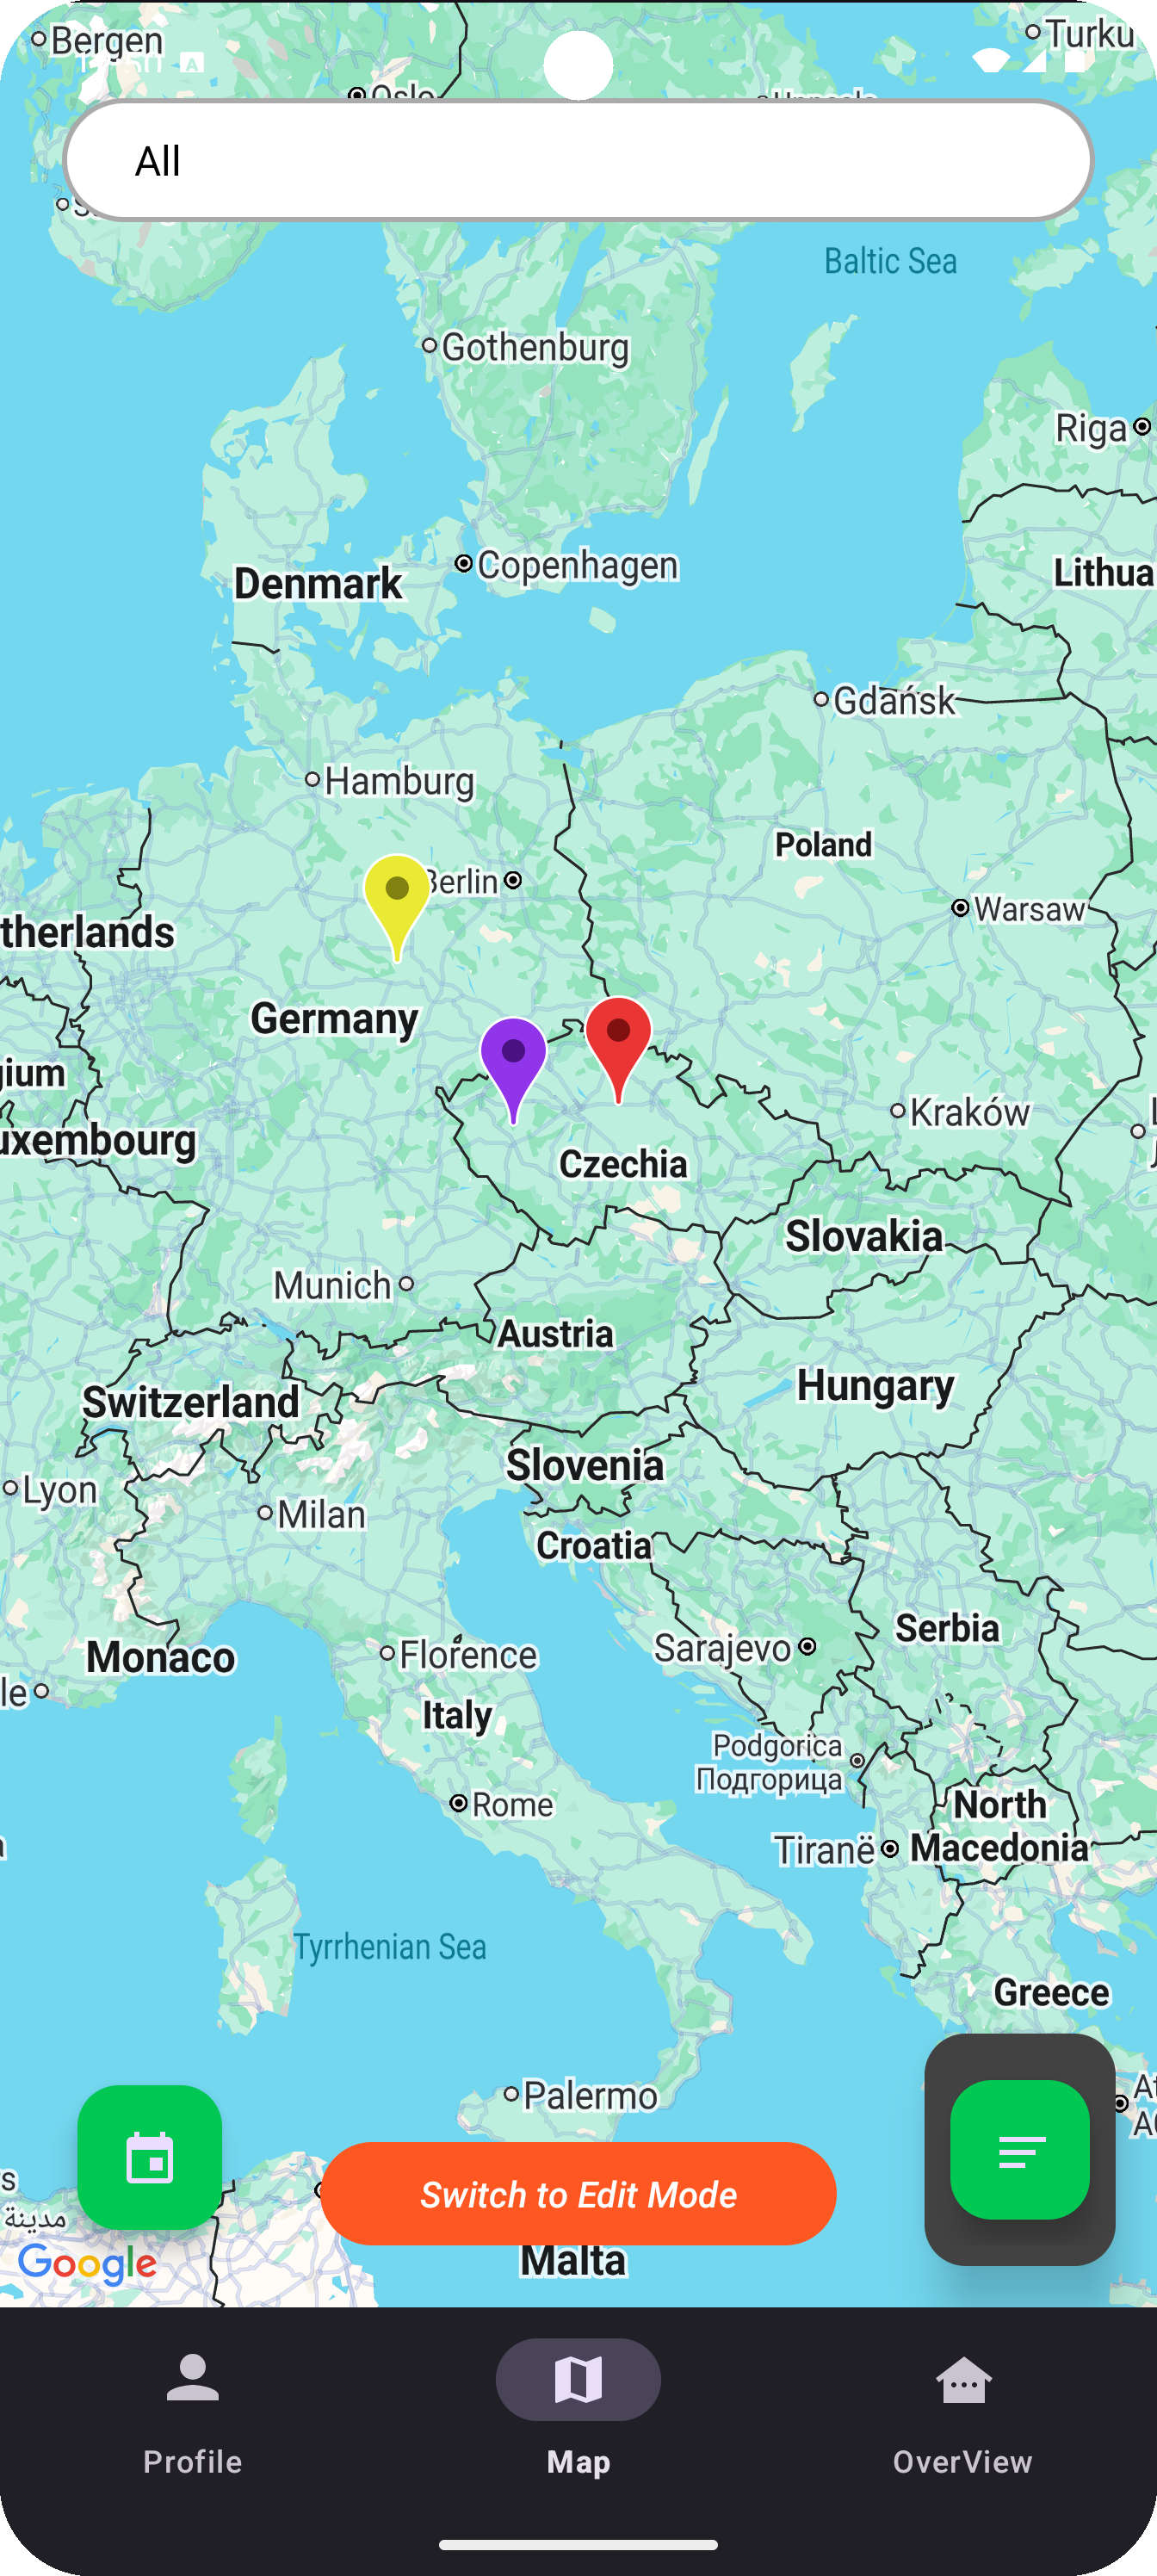
\includegraphics[height=11cm]{Images/MapsFrag.png}
    \caption{MapsFragment}
    \label{fig:Update-account}
\end{figure}

Zobrazování událostí je centralizováno do MapFragmentu. Uživatel se v mapě pohybuje pomocí tahů prstů zoom-in/out. Markery se načítají z databáze Firebase Firestore, kde jsou události uloženy. Každý marker se zobrazuje v jiné barvě podle tematického zaměření události (např. sport, hudba, festival apod.), které může vyfiltrovat. Uživatelská interakce s markery je možná pomocí jednoduchého kliknutí, které otevře okno s názvem a popisem události, a následně může uživatel přejít na detailní obrazovku události.

Součástí mapového rozhraní je filtrovací panel, který lze rozbalit a sbalit. Pomocí něj může uživatel filtrovat pouze události, kterých se účastní přátelé, filtrovat podle tvůrců, které sleduje, nebo zobrazit pouze události pořádané slavnými osobami.


Aplikace bere ohled na nezletilé, tudíž je-li uživatel příliš mladý na danou akci, automaticky se mu událost neukáže. Věkovou hranici nastavuje tvůrce akce. 

Z hlediska režimu ovládání aplikace je možné přepnout do režimu úprav, kdy může uživatel přidat vlastní událost kliknutím na libovolné místo na mapě. Tento režim skrývá všechny filtry, aby nedocházelo k rušení při přidávání nové události.

Na základě uživatelovy polohy dokáže aplikace také zvýraznit „nejlepší událost v okolí“ – pomocí algoritmu, který zohledňuje vzdálenost, oblíbená témata, historii účasti a aktivitu přátel. Lze využít lokalizování a přiblížení uživatele pomocí tlačítka od Googlu v pravém horním rohu. 

Všechny markery, které teprve budou nadcházet, se sesbírají z kolekce 'markers', kde se vezmou pouze jejich koordinace (longitude, latitude) a tématika, kvůli zbarvení.



\begin{figure}[H]
    \centering
\begin{lstlisting}[language=Java, style=myJavaStyle, caption={Metoda \texttt{loadMarkers()} – načítání a filtrování událostí}, label={lst:loadMarkers}]
private void loadMarkers() {
    firestore.collection("users").document(userId).get().addOnSuccessListener
    (userDoc -> {
        int userAge = calculateAge(userDoc.getString("birthyear"));

        firestore.collection("markers").get().addOnSuccessListener(
        queryDocumentSnapshots -> {
            googleMap.clear();
            Date now = new Date();

            for (DocumentSnapshot document : queryDocumentSnapshots) {
                String title = document.getString("title");
                String theme = document.getString("theme");
                String eventDateTime = document.getString("eventDateTime");
                int ageLimit = document.getLong("ageLimit").intValue();

                if (userAge < ageLimit) continue;
                if (!passesAllFilters(document)) continue;

                LatLng position = new LatLng(
                    document.getDouble("latitude"),
                    document.getDouble("longitude")
                );

                googleMap.addMarker(new MarkerOptions()
                    .position(position)
                    .title(title)
                    .icon(BitmapDescriptorFactory.defaultMarker(getMarkerColor(theme)))
                ).setTag(document.getId());
            }
        });
    });
}
\end{lstlisting}
\end{figure}

Tato metoda slouží k načtení všech událostí z databáze a jejich vykreslení na mapě. Před samotným zobrazením se kontroluje věk uživatele vůči minimálnímu věkovému limitu každé události, dále se aplikují filtry (např. podle data, tématu, známých osob nebo přátel), a pokud událost projde těmito podmínkami, je zobrazena na mapě.

\begin{figure}[H]
    \centering
    
\begin{lstlisting}[language=Java, style=myJavaStyle, caption={Změna barvy markeru podle tématu události}, label={lst:marker-colors}]
private float getMarkerColor(String theme) {
    if (theme == null) return BitmapDescriptorFactory.HUE_RED;

    switch (theme.toLowerCase()) {
        case "sports":
            return BitmapDescriptorFactory.HUE_BLUE;
        case "music":
            return BitmapDescriptorFactory.HUE_VIOLET;
        case "festival":
            return BitmapDescriptorFactory.HUE_YELLOW;
        case "workshop":
            return BitmapDescriptorFactory.HUE_GREEN;
        case "custom":
            return BitmapDescriptorFactory.HUE_ORANGE;
        default:
            return BitmapDescriptorFactory.HUE_RED;
    }
}
\end{lstlisting}
\end{figure}



Tato metoda vrací barvu, kterou bude mít marker na mapě podle zadaného tématu události. Pomocí konstrukce \textit{switch} se porovnává textový řetězec tématu a přiřazuje se odpovídající hodnota barvy z \texttt{BitmapDescriptorFactory}. Pokud je téma neznámé nebo chybí, použije se výchozí červená barva.
\cite{FirebaseFirestoreFilter} \cite{GoogleMapAPI}  \cite{GoogleMapsAPI} \cite{AndroidDatePicker}







\subsection*{AddMarkerActivity}

Tato aktivita slouží k přidání nové události na mapu. Uživatel se na tuto obrazovku dostane kliknutím na libovolné místo v mapě v režimu „Úpravy“. V úvodu obrazovky se zobrazí formulář, ve kterém uživatel vyplňuje název události, stručný popis, zvolenou tematiku (např. sport, hudba, festival), věkové omezení a přesný čas konání.

Formulář rovněž obsahuje datumový a časový výběr pomocí příslušných dialogových oken, které zajišťují správné formátování vstupu. Veškeré údaje jsou validovány — např. datum musí být v budoucnosti, některá pole jsou povinná.

Po úspěšném přidání je uživatel automaticky přesměrován zpět do mapového zobrazení, kde se nová událost objeví po synchronizaci jako nový marker. Logika v této aktivitě je tedy zcela propojena s databází a aktuální polohou uživatele.

Nový marker se uloží do kolekce 'markers', kde vznikne pod novým ID. \cite{AndroidDatePicker}





\subsection*{MarkerInfoActivity}

\begin{figure}[H]
    \centering
    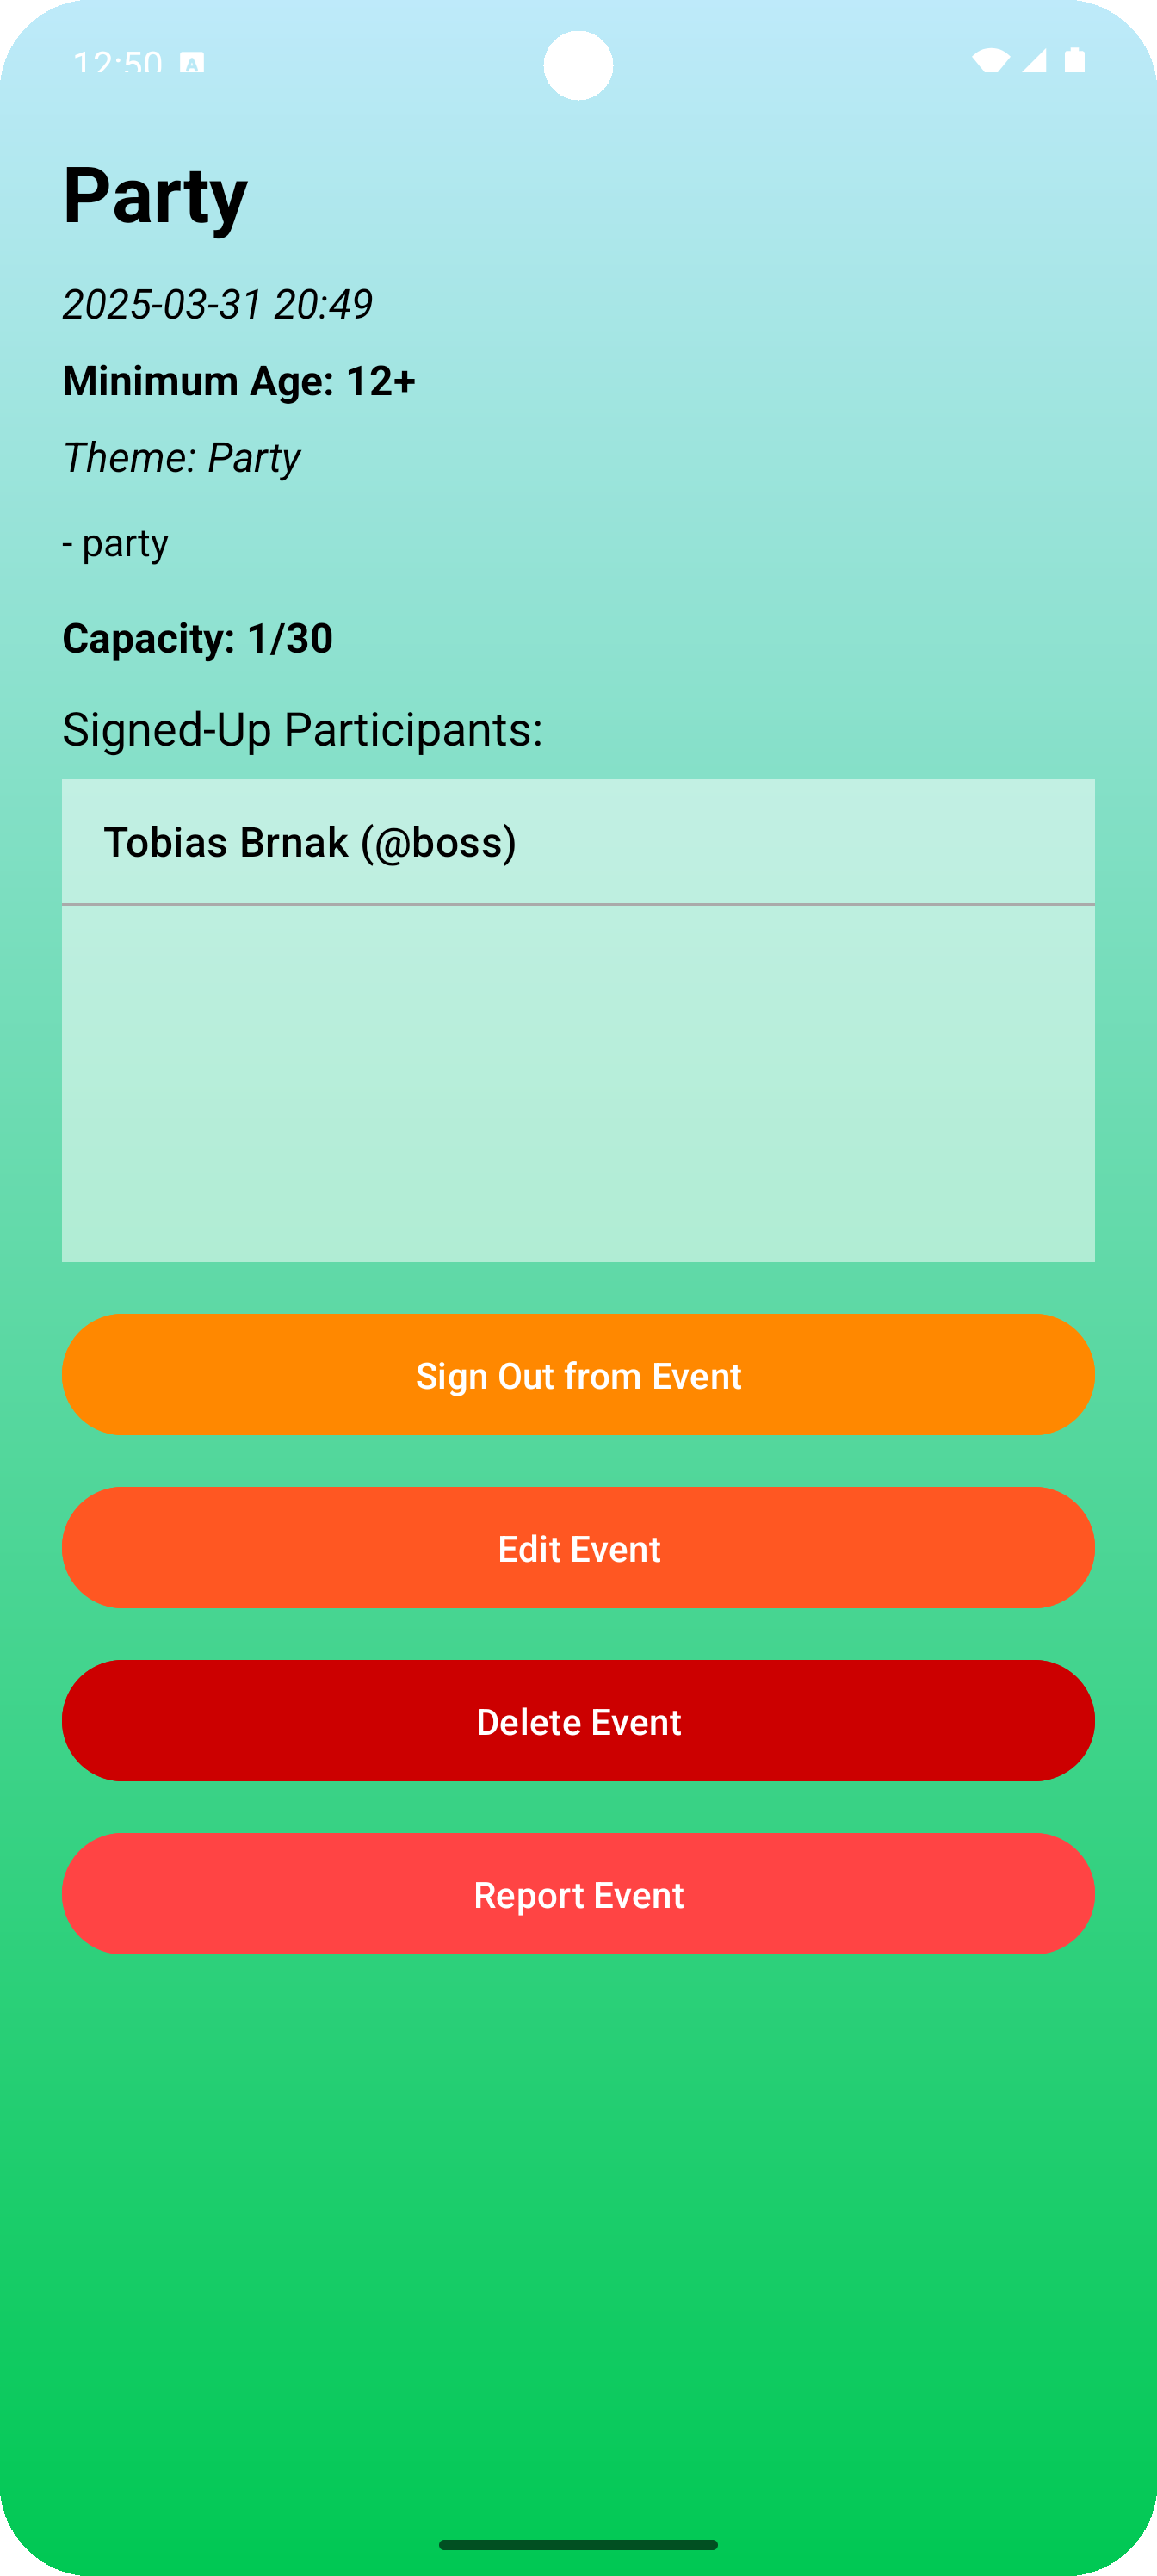
\includegraphics[height=11cm]{Images/MarkerInfo.png}
    \caption{MarkerInfoActivity}
    \label{fig:Update-account}
\end{figure}

Tato aktivita slouží jako detailní přehled konkrétní události, která byla vybrána z mapového zobrazení. Obsahuje všechny dostupné informace o události – název, popis, téma, datum a čas, věkové omezení, pozici na mapě i informace o tvůrci události.

Zobrazí se zde i možnost přihlášení se na danou událost (tlačítko „Zúčastnit se“), pokud se uživatel ještě nezúčastnil, případně možnost odhlášení. Uživatel zde také vidí, kolik dalších lidí se události účastní. Též vidí kolik míst zbývá do plné kapacity události.

Pokud je uživatel tvůrcem události, má navíc k dispozici tlačítko editace (přesměrování do 'EditMarkerActivity') a mazání události.

Získává základní informace z kolekce 'users'. Nadále je vyplní do kolonek a po uložení se použije příkaz aktualizace databáze.

Tato aktivita vyhledá ID markeru v kolekci 'markers' a vypíše všechna informace. Seznam přihlášení se vezme z kolekce 'event\_guest\_list', kde pod stejným ID jsou napsání uživatelé, kteří se na akci přihlásili.






\subsection*{EditMarkerActivity}

Editační aktivita slouží ke správě již existující události, kterou vytvořil sám uživatel. Přístup k této obrazovce je možný skrze detail události `MarkerInfoActivity` pouze v případě, že je aktuálně přihlášený uživatel zároveň tvůrcem dané události.

Zobrazuje předvyplněný formulář s údaji o události, jako je název, popis, datum a čas, tematické zaměření a případné věkové omezení. Uživatel může libovolné pole upravit, a následně změny uložit. Náhled události se po editaci aktualizuje i v mapovém zobrazení.

Tato aktivita rovněž umožňuje zrušit událost úplným smazáním. Bezpečnostní kontrola zajišťuje, že danou událost může upravovat a mazat výhradně její vlastník.

Získává základní informace z kolekce 'markers'. Nadále je vyplní do kolonek a po uložení se použije příkaz aktualizace databáze.





\subsection*{ProfileFragment}

\begin{figure}[H]
    \centering
    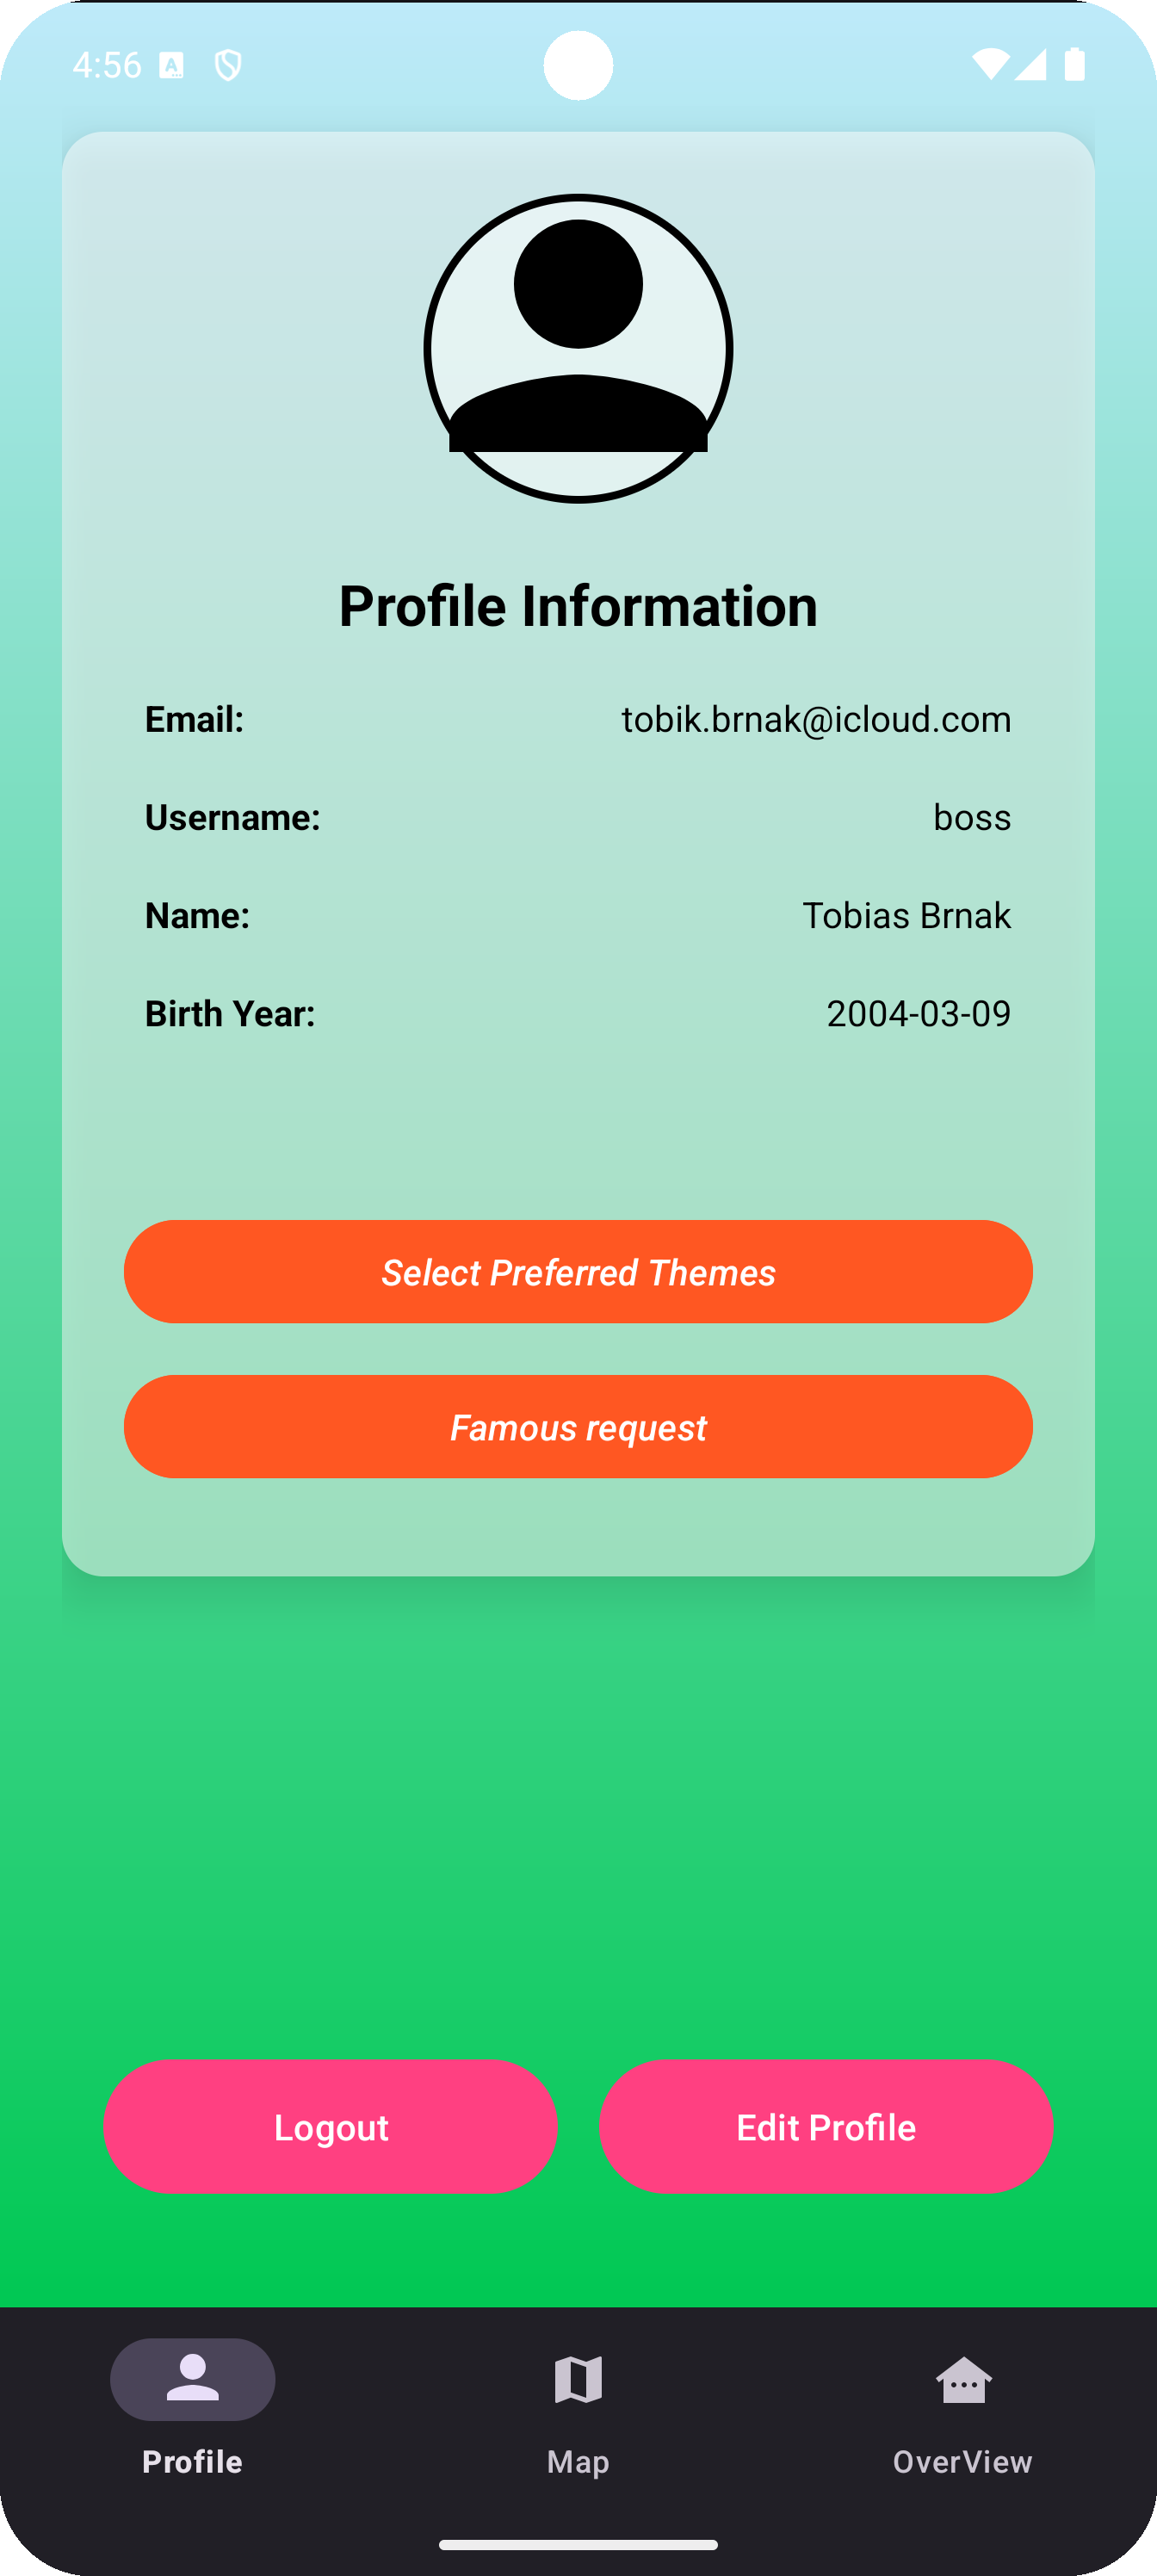
\includegraphics[height=11cm]{Images/Profile_frag.png}
    \caption{ProfileFragment}
    \label{fig:Update-account}
\end{figure}

Tento fragment slouží jako uživatelský profil. Po načtení fragmentu se zobrazí informace přihlášeného uživatele - přezdívka (username), jméno, příjmení, e-mail a rok narození. Tyto informace jsou zobrazeny formou přehledného seznamu v kartičce.

Uživatel má možnost upravit své osobní údaje kliknutím na tlačítko Editovat profil, které ho přesměruje do aktivity 'EditProfileActivity', odhlásit se z aplikace pomocí tlačítka Odhlásit se, které spustí návrat na přihlašovací obrazovku, nebo si vybrat oblíbená témata událostí kliknutím na tlačítko Vybrat témata, což otevře výběrové dialogové okno se seznamem témat.

Pokud je uživatel slavný (\textit{Famous}), je jeho profilový obrázek automaticky změněn na ikonku korunky. Tím je vizuálně odlišena jeho identita.

'ProfileFragment' vyhledá ID shodné s přihlášeným uživatelem a vypíše dané informace, které se následně zobrazí.



\subsection*{EditProfileActivity}

Tato aktivita umožňuje uživateli upravit své základní osobní údaje. Po načtení se automaticky předvyplní stávající data – přezdívka (username), jméno, příjmení a rok narození. 

Uživatelské rozhraní obsahuje vstupní pole pro každou informaci a tlačítko pro potvrzení změn. Při odeslání dat proběhne kontrola platnosti zadaných údajů (např. zda nejsou prázdné) a následně dojde k jejich aktualizaci v dokumentu přihlášeného uživatele.

Získává základní informace z kolekce 'users'. Nadále je vyplní do kolonek a po uložení se použije příkaz aktualizace databáze.



\subsection*{OverviewFragment}

Tento fragment slouží jako přehled účasti uživatele. Uživatel zde najde 4 hlavní sekce seznamů:
\begin{itemize}
    \item Události, které uživatel vytvořil a budou se konat – bere je z kolekce 'markers', kde zjišťuje, zda se schoduje 'userID' s ID přihlášeného uživatele.
    \item Události, na které vytvořil a již se konaly – dotázání se na kolekci 'user\_owner\_arch'
    \item Události, na které se přihlásil v budoucnu – dotázání se na kolekci 'user\_events'
    \item Události, na které se přihlásil v minulosti – dotázání se na kolekci 'user\_arch'

\end{itemize}

Každá událost je zobrazena jako jednoduchý seznam s názvem a datem. Kliknutím na konkrétní událost se uživatel přesměruje do detailu události (`MarkerInfoActivity`), kde si může zobrazit detaily nebo se z události odhlásit.

Tento fragment je vhodný pro rychlou orientaci v historii a plánech uživatele.
\cite{FirebaseFirestoreFilter} 







\subsection*{FollowingActivity}

\begin{figure}[H]
    \centering
    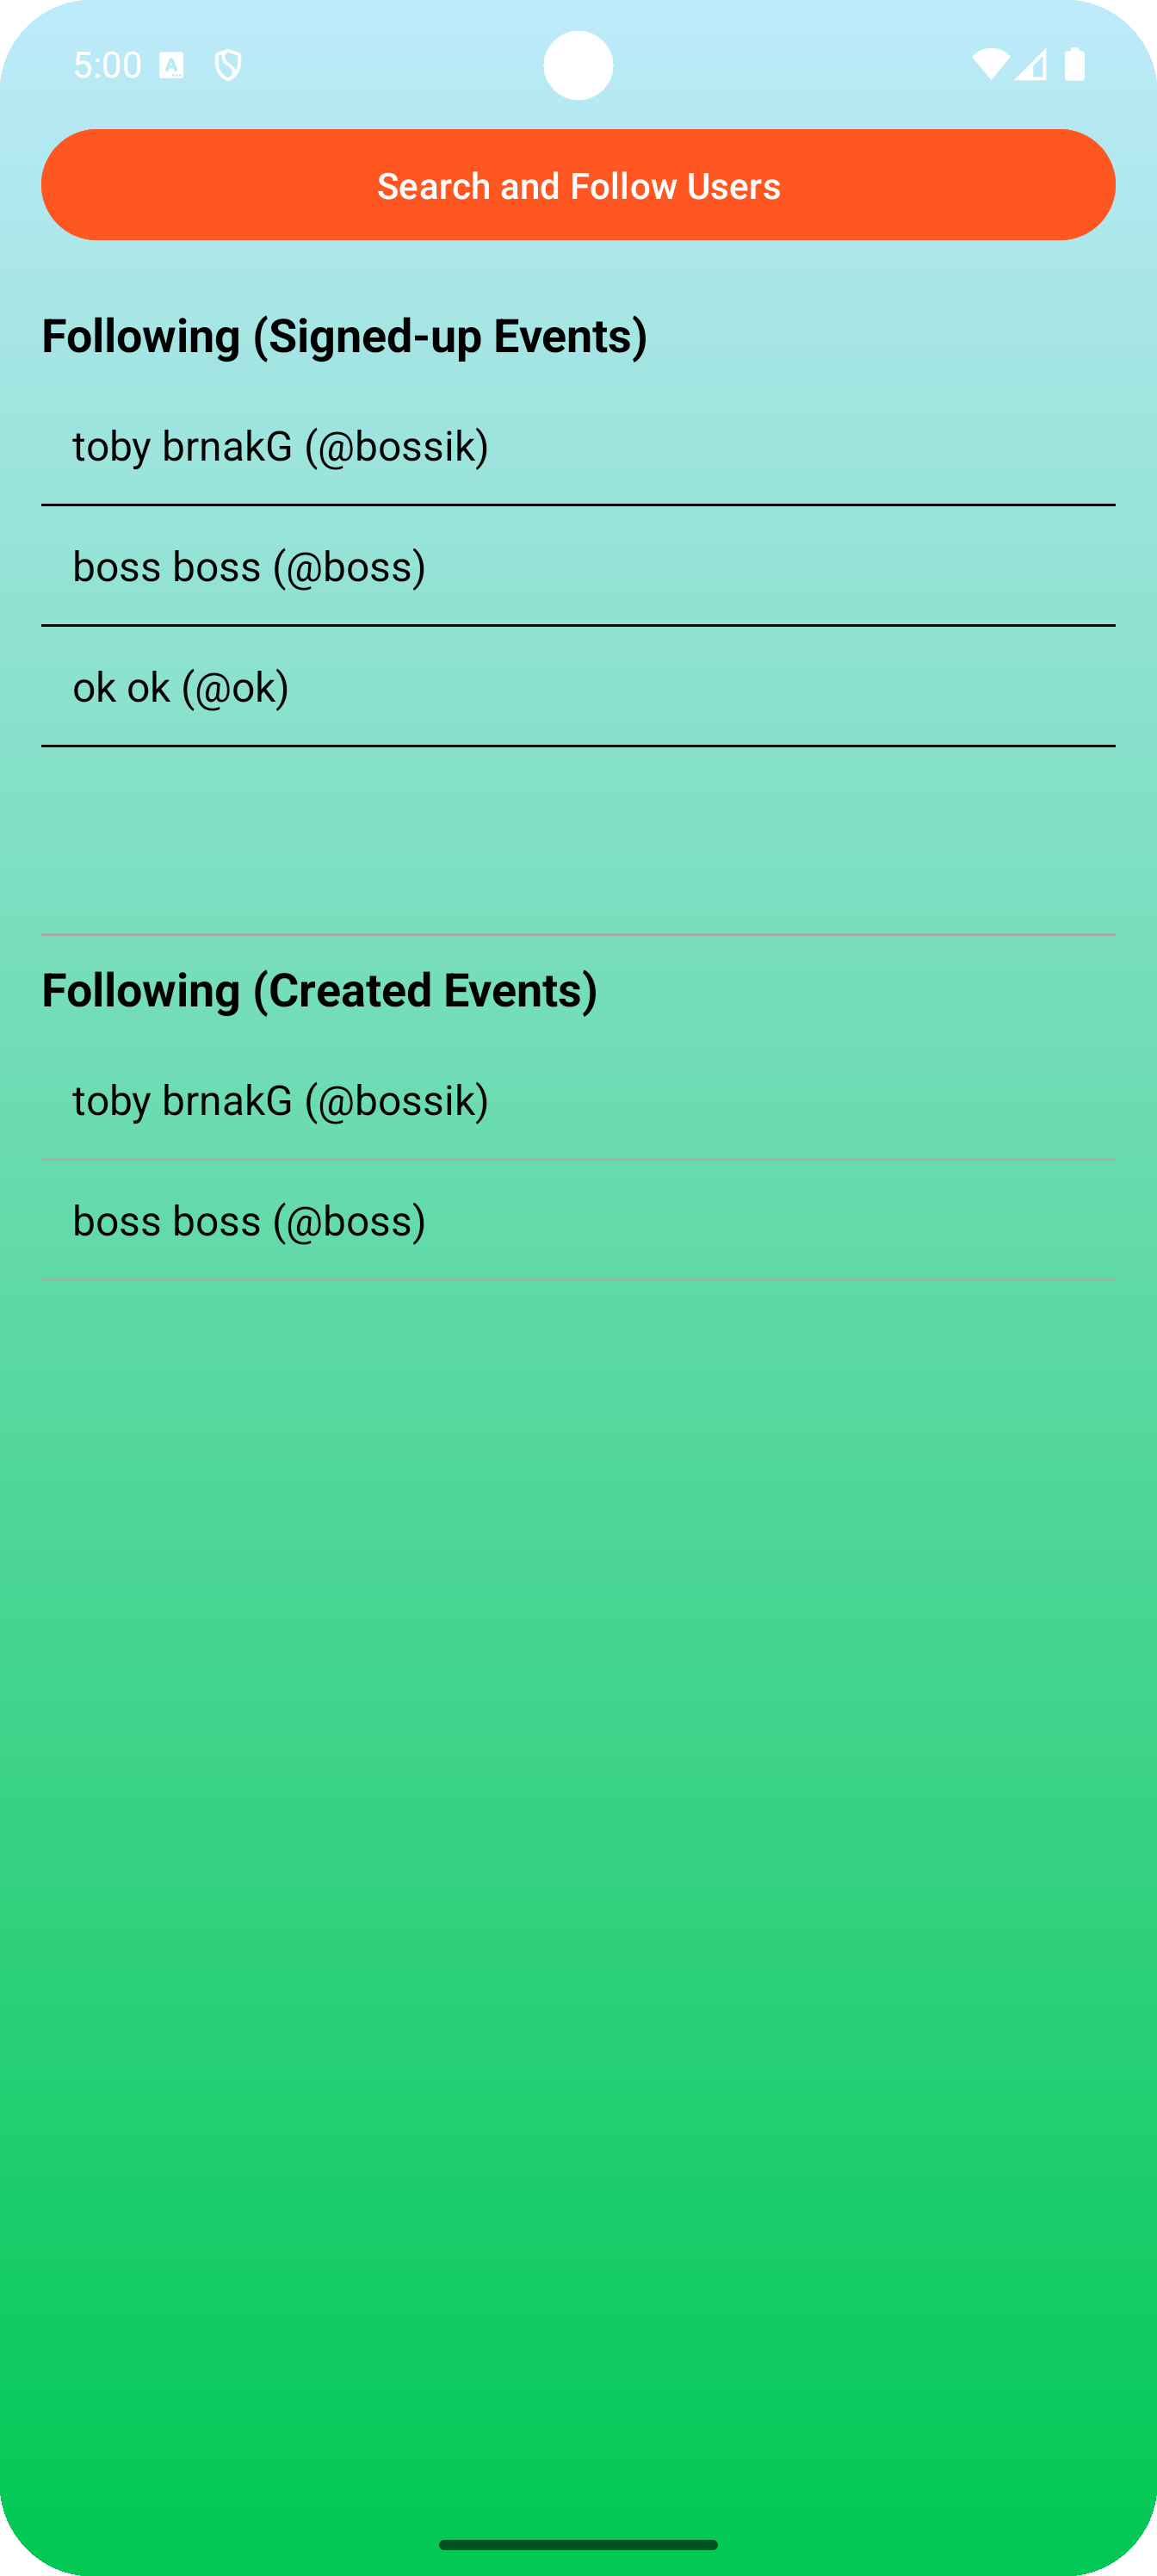
\includegraphics[height=11cm]{Images/Following_activity.png}
    \caption{FollowingActivity}
    \label{fig:Update-account}
\end{figure}

Aktivita umožňuje zobrazit seznam uživatelů, které daný uživatel sleduje, a to jak v roli tvůrců, tak přihlášených přátel. Aktivita je vybavena dvěma seznamy uživatelů. Sbírá data z kolekce 'user\_signup\_follow' a 'user\_create\_follow'







\subsection*{SearchUsersActivity}

\begin{figure}[H]
    \centering
    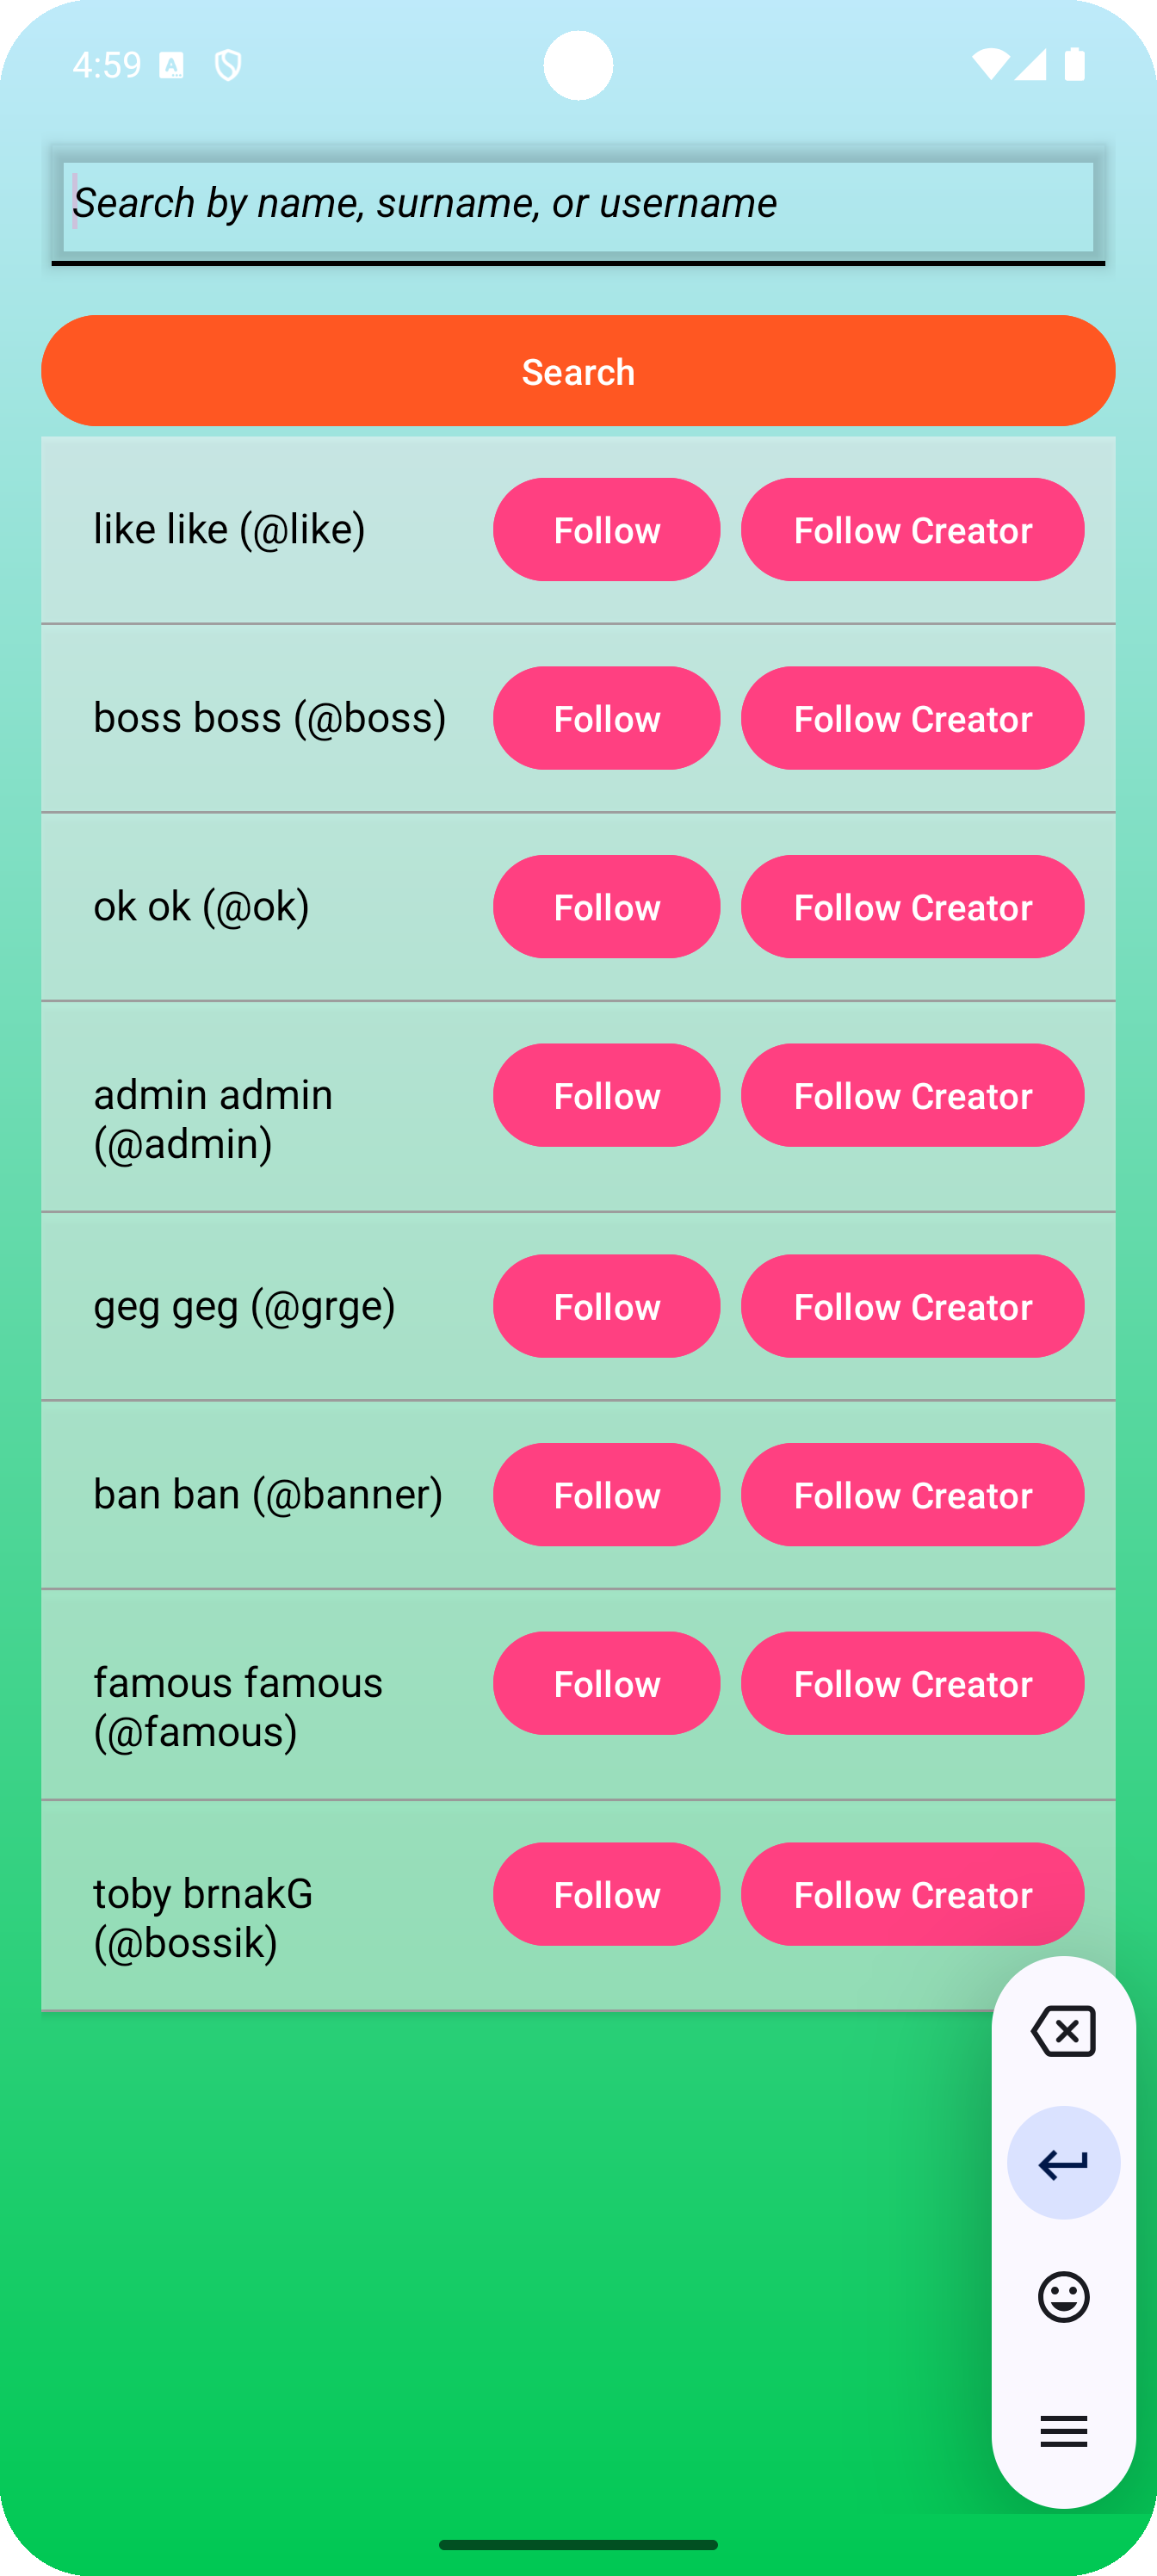
\includegraphics[height=11cm]{Images/Search_users_Following.png}
    \caption{SearchUsersActivity}
    \label{fig:Update-account}
\end{figure}

Tato aktivita slouží k vyhledávání ostatních uživatelů v databázi. Po zadání jména nebo přezdívky se vyfiltrují odpovídající výsledky. U každého uživatele má uživatel možnost zobrazit základní informace, začít sledovat daného uživatele z důvodu, kam se přihlašuje (Follow), nebo začít sledovat daného uživatele z důvodu jeho tvorby (Follow creator).


Načítání uživatelů je pomocí adaptéru ve třídě 'UserAdapter', která dále využívá další třídu 'User' shrnující základní informace o uživateli. Filtrování funguje pomocí dotázání se příkazem \textit{.whereEqualTo()}. Po stisknutí jednoho z tlačítek se informace zapíše do kolekce      'user\_signup\_follow' nebo 'user\_owner\_follow' pod dokument ID přihlášeného uživatele, uživatel, kterého zaklikne, že chce sledovat.
\cite{FirebaseFirestoreFilter}






\subsection*{AdminProfile.java}

Tato aktivita představuje hlavní rozhraní pro administrátora aplikace. Po přihlášení jako administrátor je uživatel přesměrován právě sem. Od této aktivity se administrátor může dostávat do jiných odvětví.

Zde má administrátor možnost kliknout na tlačítko, kde se zobrazí přehled všech uživatelů aplikace 'AdminUserList'a nebo se může z aplikace odhlásit.




\subsection*{AdminUserList.java}

Třída slouží pro získání a zobrazení seznamu všech registrovaných uživatelů aplikace.

Uživatelé jsou zobrazováni v přehledném seznamu. Seznam je interaktivní – kliknutím na položku je administrátor přesměrován na detailní zobrazení konkrétního uživatele.

Součástí je již využitá základní logika filtrování a aktualizace dat. Funguje na stejném principu jako aktivita 'SearchUsersActivity'.









\subsection*{AdminUserDetails.java}

Tato aktivita zobrazí detailní informace o konkrétním uživateli, vybraném z předchozího seznamu. Zobrazuje všechny informace z databáze.


Administrátor zde může pomocí přepínačů měnit atributy uživatele – například přidělit mu roli admina, slavné osoby nebo ho zabanovat. Po úpravách jsou změny ihned synchronizovány s Firestore databází.

Po kliknutí na kartičku se vyhledá v kolekci 'users' id dokumentu shodný s ID uživatelem, na který bylo kliknuto.

\begin{figure}[H]
    \centering
    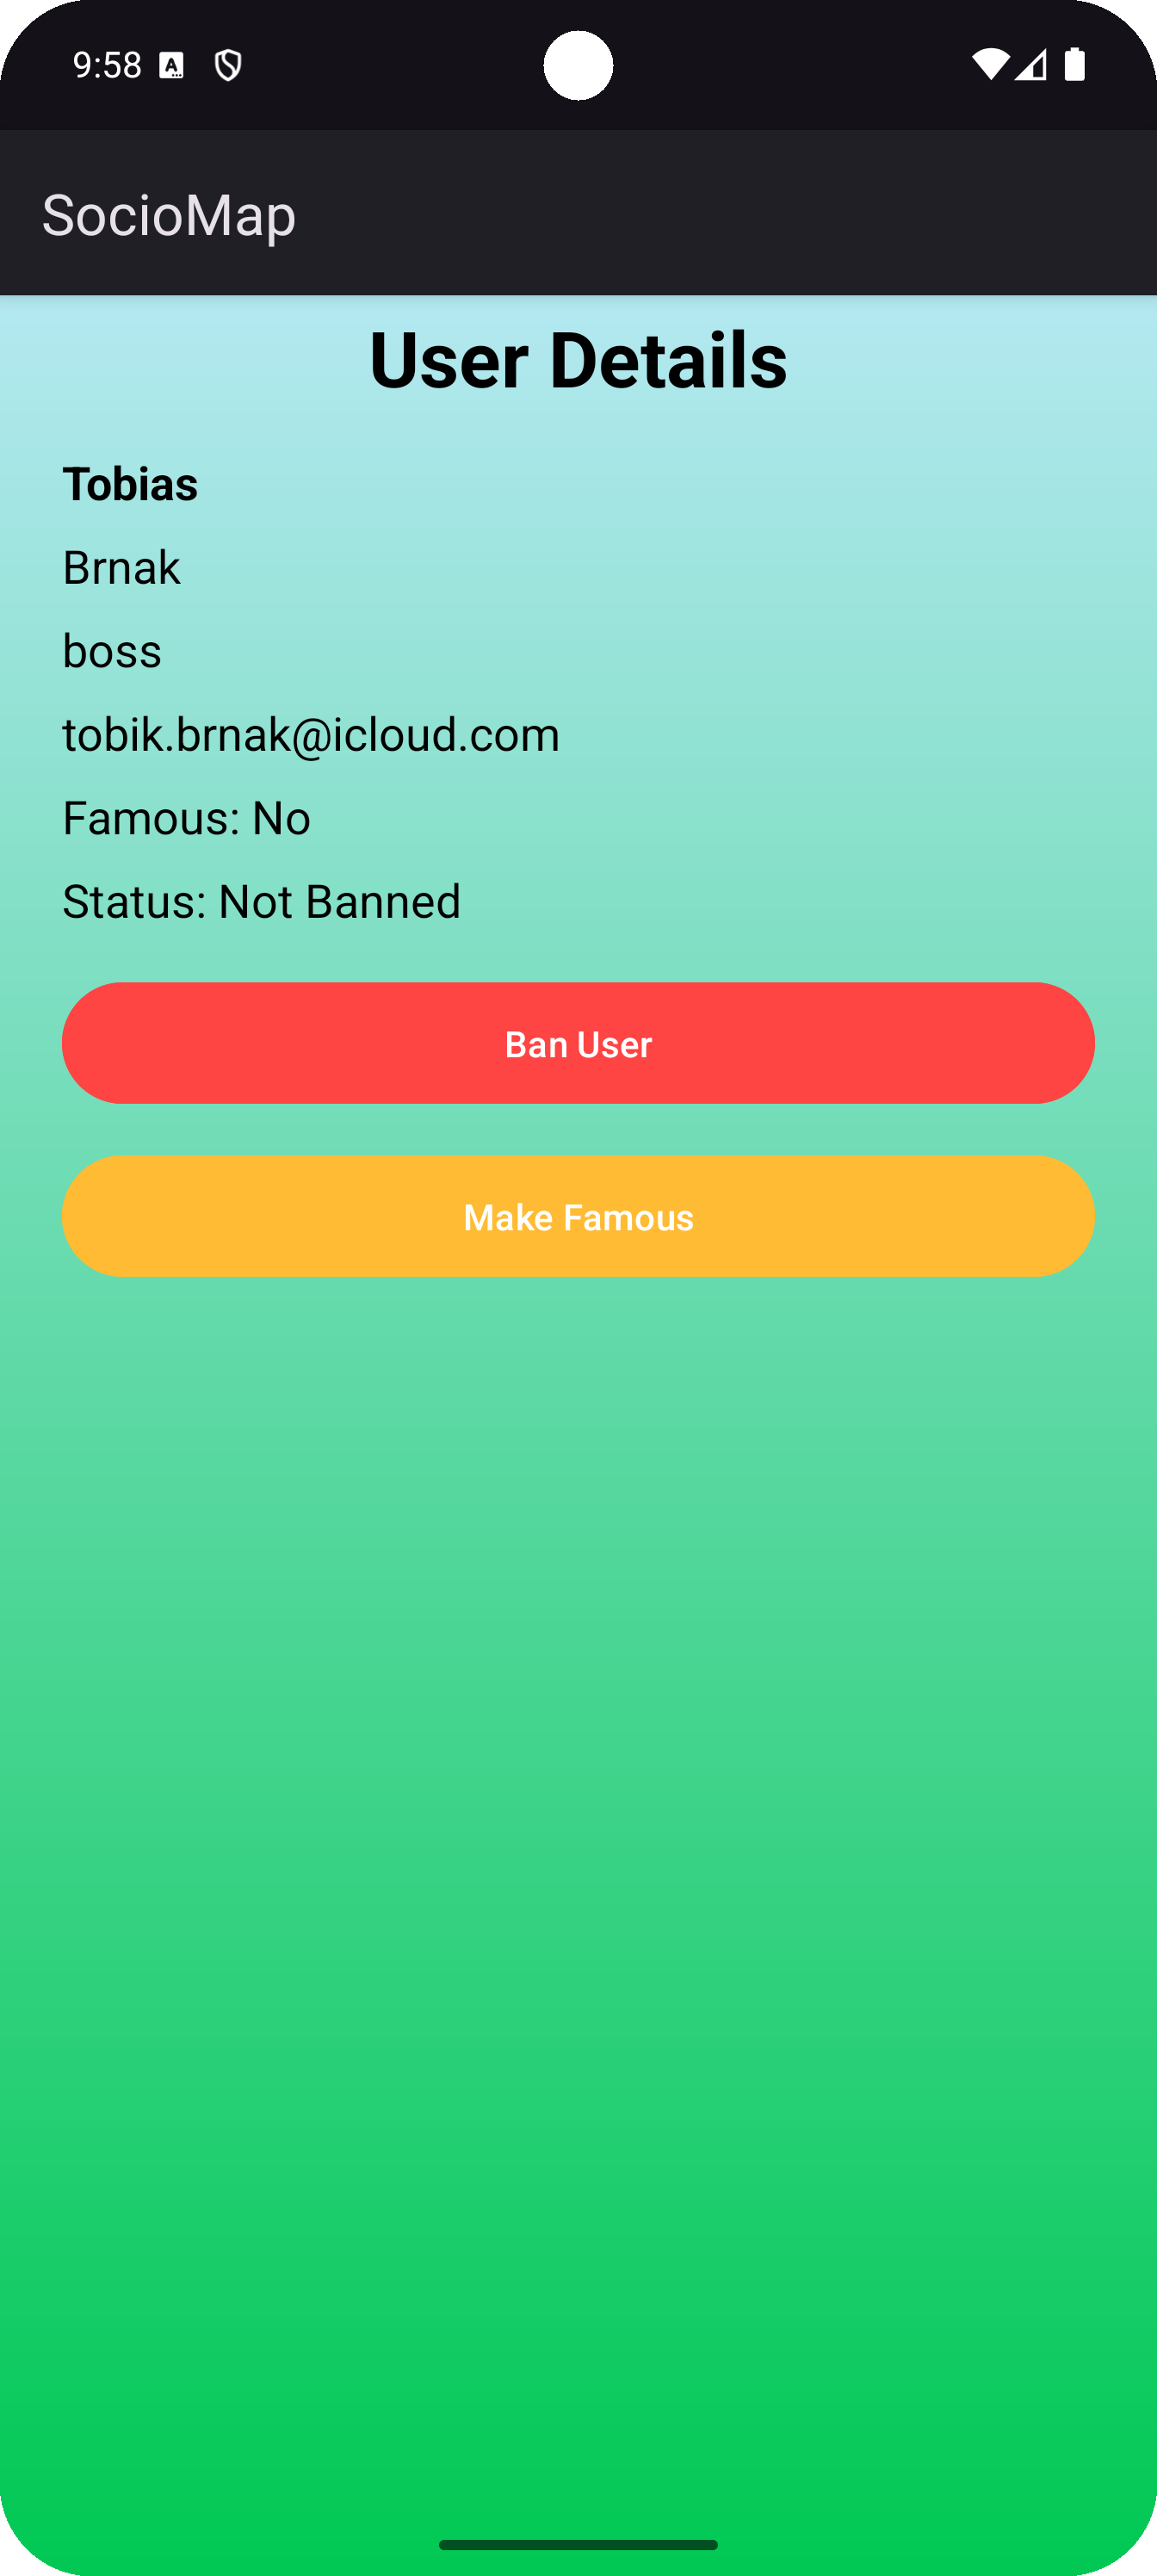
\includegraphics[height=11cm]{Images/AdminDetail.png}
    \caption{AdminUserDetails}
    \label{fig:Update-account}
\end{figure}








\subsection{Role a oprávnění uživatelů}

Aplikace SocioMapa rozlišuje tři základní typy uživatelů, kteří mají rozdílná oprávnění:

\begin{itemize}
    \item \textbf{Běžný uživatel} – může plně využívat funkcionality aplikace, jako je přidávání přátel, přihlašování se na události, vytváření vlastních událostí a filtrování záznamů v mapě. Má přístup pouze ke svým údajům a událostem.
    
    \item \textbf{Slavný uživatel (Famous)} – je vizuálně zvýrazněn pomocí speciálního designu. Na mapě se jeho události zobrazují pomocí odlišného stylu (např. korunka, výraznější barva markeru), což zvyšuje jejich viditelnost pro ostatní uživatele. 
    
    \item \textbf{Administrátor (Admin)} – má rozšířená oprávnění pro správu systému. Může:
    \begin{itemize}
        \item nastavovat status \texttt{isFamous} jiným uživatelům,
        \item blokovat účty pomocí příznaku \texttt{ban},
        \item zobrazovat podrobné informace o všech uživatelích.
    \end{itemize}
\end{itemize}

\begin{figure}
    \centering
    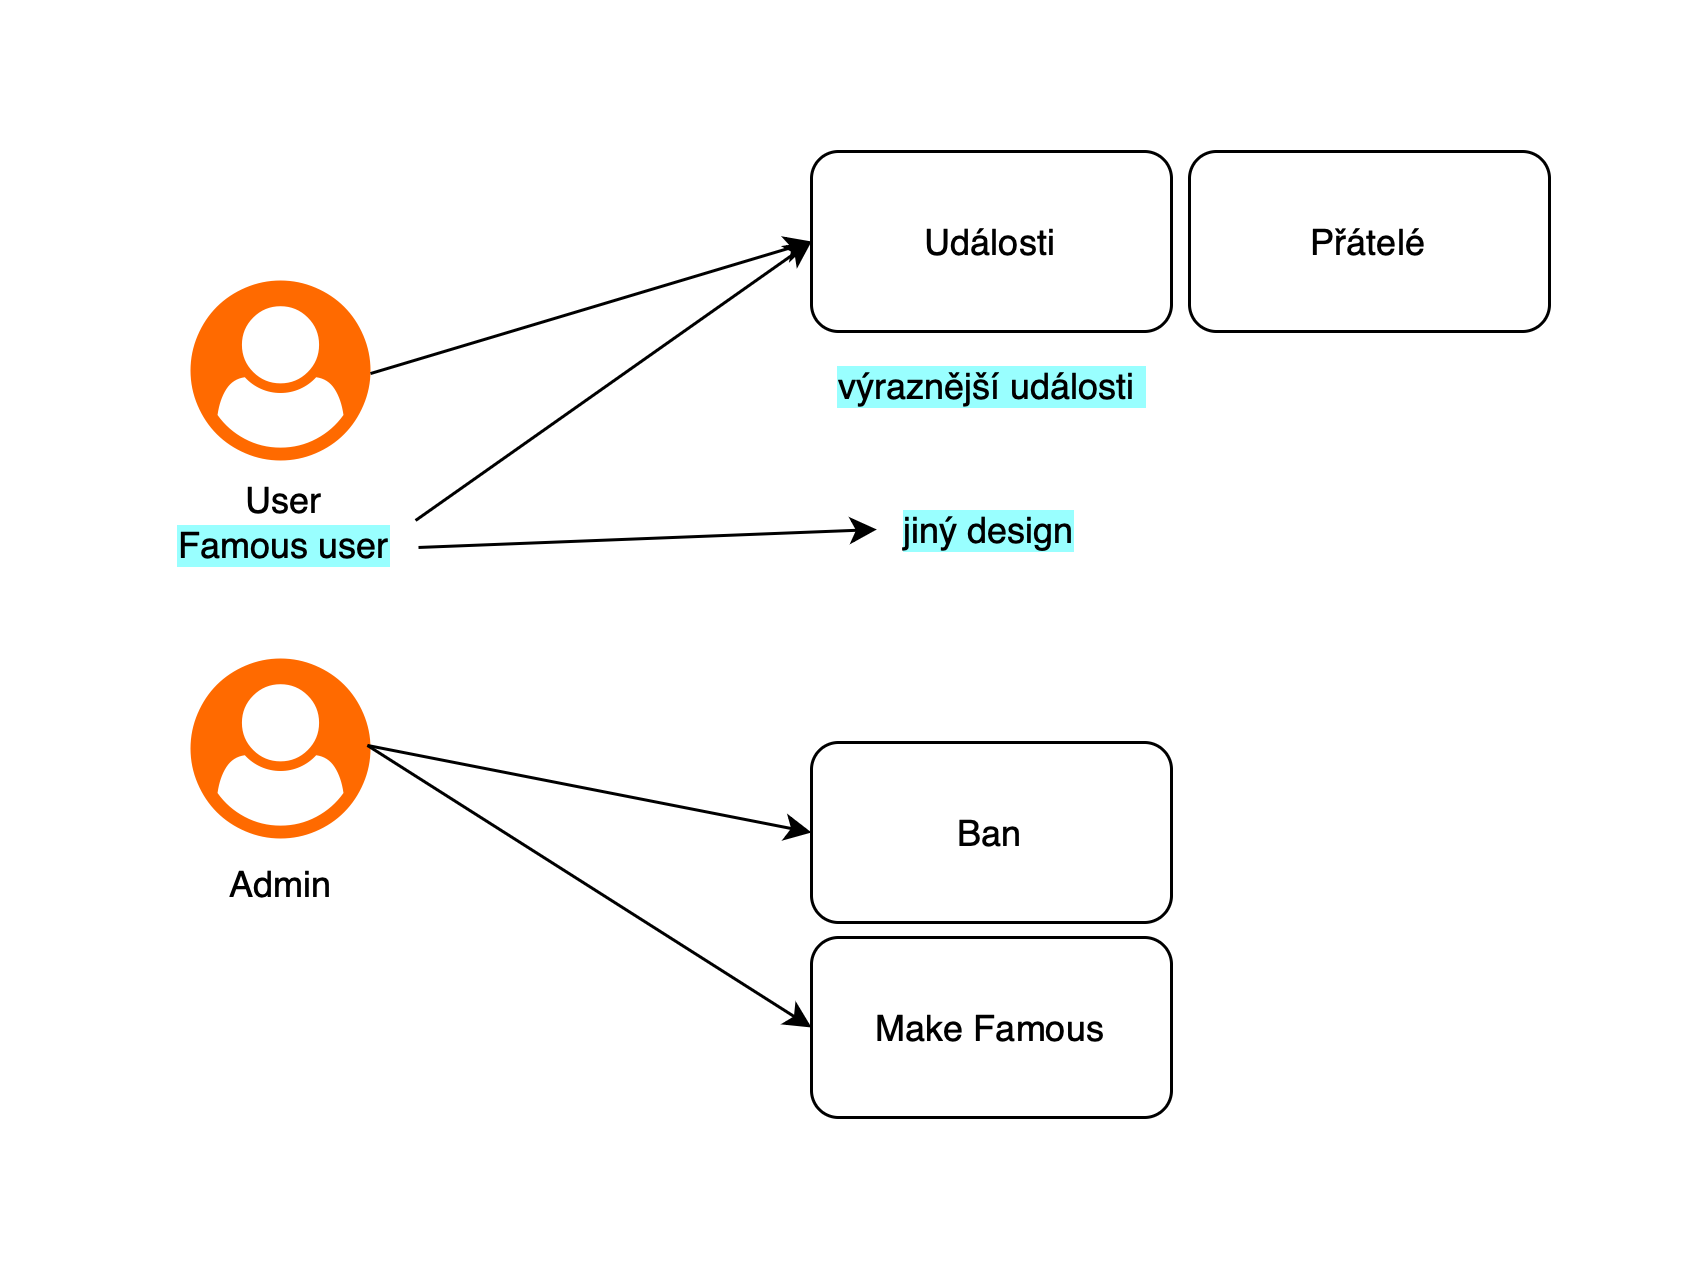
\includegraphics[width = \textwidth]{Images/User_relations.drawio.png}
    \caption{Role uživatele a jejich vztahy v systému}
    \label{fig:Update-account}
\end{figure}

Na obrázku je znázorněno, jak běžný uživatel a slavný uživatel interaguje s přáteli (sleduje je a vidí jejich aktivity) a s událostmi (vytváří je nebo se na ně přihlašuje). Admin uživatel smí interagovat s proměnnými jako jsou \textit{ban} a \textit{isFamous}.







\chapter{Program}

\section{Pomocné třídy}


\subsection*{User.java}

Třída 'User' slouží jako datový model pro uživatele aplikace. Obsahuje základní atributy, jako je identifikátor uživatele (userId), přezdívka (username), jméno (name) a příjmení (surname). Tento model je využíván při práci s databází Firestore – jak při získávání údajů o uživateli, tak při jejich ukládání. Umožňuje přehlednější manipulaci s daty v rámci kódu a zajišťuje jednotnou strukturu uživatelských informací napříč aplikací.


\subsection*{UserListAdapter.java}

Tato třída je 'RecyclerView.Adapter', která slouží k zobrazení seznamu uživatelů v rozhraní administrátora a v aktivitě 'SearchUsersActivity'. Každý uživatel je vykreslen jako samostatná položka se základními informacemi (jméno, příjmení, přezdívka) dle předlohy ze třídy 'User'.

Adapter propojuje data z databáze s vizuální reprezentací v seznamu. Při kliknutí na položku je vyvolán listener, který otevře detail konkrétního uživatele v aktivitě 'AdminUserDetails'.






\subsection*{NetworkChangeReceiver.java}

Tato komponenta je zaregistrována jako \texttt{BroadcastReceiver}, který sleduje stav připojení k internetu. 

Pokud dojde ke ztrátě připojení, je uživatel upozorněn vizuálním prvkem (ikona, hláška) a některé interakce (např. přihlášení, registrace) jsou dočasně zakázány. Tudíž se uživatel nemůže přihlásit.

Třída preventivně zakazuje vstoupit do aplikace bez připojení k internetu, jelikož bez přístupu k databázi, nemá aplikace smysl.




\subsection*{EmailSender.java}

Tato pomocná třída umožňuje odesílání e-mailů pomocí SMTP protokolu. Je využívána zejména pro správu systému ze strany administrátora – např. při nahlášení události nebo informování uživatelů. Výjimkou je změna statusu z běžného uživatele na slavného, kdy uživatel obdrží email s informací, že se stává slavným.

Třída obsahuje základní SMTP konfiguraci a metody pro vytvoření zprávy a její odeslání. Připojuje se k e-mailové službě, jako je Gmail, a zabezpečuje přenos přihlašovacích údajů i obsahu zprávy.

Používá JavaMail API a pracuje na pozadí, aby neblokovala hlavní UI vlákno.

\cite{JavaDocs} \cite{MapTapStackoverflow}




\section{Firebase}

Pro realizaci backendové části jsem zvolil platformu Firebase, konkrétně služby Firestore, Firebase Authentication. Vzhledem k povaze aplikace – tedy zaměření na víceuživatelské prostředí a potřebu rychlé synchronizace dat – nebyla použita lokální SQL databáze. Lokální databáze by neumožnila správu účtů napříč zařízeními, a při přihlášení z jiného zařízení by uživatel neměl přístup ke svým událostem či osobním údajům. Firestore zároveň umožňuje práci v reálném čase, díky čemuž se změny (např. vytvoření nebo úprava události) okamžitě promítnou všem uživatelům.

\subsection{Struktura databáze (Firestore Collections)}

Databáze je tvořena několika kolekcemi, z nichž každá má specifický účel:

\begin{itemize}
  \item \textbf{users} – obsahuje základní údaje o uživatelích (jméno, příjmení, přezdívka, rok narození, email, typ účtu – admin/slavný, priorizované tématiky) [String = (username, name, surname, email, birthday) Boolean = (isFamous, isAdmin, ban) List = (preferredThemes)]. Dokument vytváří ID uživatele po úspěšné registraci.
  \item \textbf{markers} – aktivní události, které se zobrazují na mapě. Každý dokument v kolekci `markers` obsahuje informace (název, popis, souřadnice, datum a čas, věkové omezení, tematické zaměření a ID autora, kapacitu, maximální kapacita). [Number = (ageLimit, currentAttendees, latitude, longitude, maxCapacity)
  String = (description, eventDateTime, theme, title, userId)] Dokument nese nově vytvořený ID markeru.
  \item \textbf{markers\_arch} – archiv událostí, které již proběhly. Pokud akce již proběhla, bude přesunuta sem.
  \item \textbf{user\_events} – seznam událostí, na které se uživatel přihlásil. [List = (events)] Dokument nese ID uživatele.
  \item \textbf{user\_owner\_arch} – archiv událostí vytvořených konkrétním uživatelem. [List = (events)] Dokument nese ID uživatele.
  \item \textbf{user\_sign\_up\_follow} – seznam uživatelů, jejichž účast na akcích sleduji. [List = (following)] Dokument nese ID uživatele.
  \item \textbf{user\_create\_follow} – seznam uživatelů, jejichž tvorbu akcí sleduji. [List = (following)] Dokument nese ID uživatele.
  \item \textbf{event\_guest\_list} – seznam přihlášených uživatelů pro konkrétní událost. [List = (users)] Dokument nese ID markeru.
\end{itemize}



Aplikace, jak již bylo zmíněno, využívá komunikaci na bázi endpointů pro dotazování do databáze. Pro filtrování dat je použit příkaz \textit{.whereGreaterThan("latitude", userLocation.latitude - latOffset)}, který vrátí dokumenty s hodnotou větší než zadaná hodnota, nebo .whereIn("category", Arrays.asList("sports", "music", "tech")), který vrátí dokumenty odpovídající jedné z hodnot v seznamu. Odkaz na kód je dostupný v kapitole \hyperref[sec:structure]{Struktura a propojení komponent}.

\cite{FirebaseDocs} \cite{FirebaseQuickStart} 

.





\subsection{Pravidla zabezpečení (Security Rules)}

Pro zajištění bezpečnosti a správné správy dat byla v databázi Firestore nastavena pravidla, která omezují přístup pouze na oprávněné a přihlášené uživatele. Pravidla zajišťují, že číst a zapisovat události v kolekci 'markers' může pouze jejich vlastník. Stejné omezení platí i pro přístup k uživatelským dokumentům v kolekci 'users', kde má každý uživatel přístup výhradně ke svým vlastním datům. Obdobně je chráněna kolekce 'user\_events', kde může uživatel pracovat pouze se svými událostmi. Dále jsou nastavena obecná pravidla, která umožňují pouze přihlášeným uživatelům číst a zapisovat, ale neumožňují hromadný výpis celé kolekce, čímž je zabráněno případnému zneužití nebo stahování všech dokumentů najednou.

Tato pravidla zajišťují, že pouze přihlášení uživatelé mají přístup k datům. Uživatel může upravovat nebo číst pouze svůj vlastní dokument. Nikdo nemůže stáhnout celou kolekci dokumentů najednou, což je zajištěno pravidlem \textit{List: if false}. Každý může číst veřejné informace o událostech, ale upravovat je smí pouze jejich autor.

\cite{FirebaseDocs}



\subsection{Autentizace uživatelů}

Firebase Authentication je využita pro přihlašování, registraci a ověření emailu. Prozatím je využívána pouze metoda 'Email a heslo'– uživatel se zaregistruje se svým emailem a heslem. Následně je vyžadována verifikace emailu. Poté je vytvořen nový dokument ve Firebase.

Dále byly nastaveny restrikce na heslo. Heslo požaduje velká a malá písmena, znak, číslici a délku minimálně 8 znaků. Počet přihlášení za hodinu je omezen na 10 pokusů.
\cite{FirebaseDocs}






\section{Vlastní design}

V celé aplikaci byl použit vlastní design s důrazem na vizuální konzistenci a unikátní uživatelské rozhraní. Místo výchozích systémových prvků byly navrženy vlastní komponenty. Designový prvek filtrační panel na mapě byl graficky upraven tak, aby neomezil zorné pole. Zároveň byl doplněn o animaci pro plynulé rozbalení a sbalení, což zlepšuje uživatelský dojem.

Seznam uživatelů (tzv. UserList) byl taktéž navržen jako vlastní layout. Každý uživatel je zobrazen v kartičce se zaobleným pozadím, odlišeným tlačítkem pro sledování a celkově přehledným uspořádáním textu. Pro dosažení tohoto vzhledu byly využity vlastní XML soubory s barevným přechodem, úpravou fontů a ohraničením.
\cite{MaterialComponents}







\section{Markery – události}

Události jsou reprezentovány jako markery na mapě a jsou uloženy v kolekci \texttt{markers} ve Firebase Firestore. Každý marker obsahuje základní informace jako název, popis, lokaci, datum a čas události, téma, věkové omezení a příznak popularity (\texttt{isFamous}).

\subsection{Vývoj struktury událostí}

Na začátku jsem zvažoval více způsobů, jak data o událostech ukládat – například jestli mít každého uživatele jako hlavní dokument a jeho události jako podkolekci. Nakonec jsem se rozhodl pro samostatnou kolekci 'markers', protože je přehlednější dotazovat všechny události napříč uživateli. Zároveň je snadnější filtrovat podle témata, datumu nebo věku. Tento přístup umožňuje efektivnější vyhledávání a doporučování událostí bez nutnosti procházení dalších kolekcí a také nabízí možnost využít více úložišť.

Informace o přihlášených uživatelích jsem přesunul do samostatné kolekce 'event\_guest\_list' a informace o vlastních vytvořených událostech do 'user\_owner\_arch'. Tento rozklad umožňuje lepší přehlednost, oddělení funkcí a větší kapacitu pro data.


\subsection{Algoritmus doporučené události}

Pro doporučení ideální události v okolí jsem implementoval algoritmus, který zohledňuje polohu uživatele, vzdálenost událostí, oblíbená témata a také počet přihlášených přátel. Cílem je doporučit nejbližší událost, která má co největší šanci uživatele zaujmout. Na mapě je tato událost zvýrazněna odlišnou barvou a zobrazí se popisek s názvem akce doprovázený popisem o akci.

Algoritmus nejprve získá aktuální polohu uživatele pomocí GPS souřadnic. Poté načte z kolekce 'user\_signup\_follow' seznam uživatelů, které aktuální uživatel sleduje. Následně stáhne všechny události (markery) v okruhu 7 km podle zeměpisné šířky a délky.

Každé události se vypočítá skóre na základě několika faktorů: vzdálenosti od uživatele, podílu přihlášených přátel (čím více, tím lépe) a shody s oblíbenými tématy uživatele (pokud se téma shoduje, skóre se sníží). Nakonec se událost s nejnižším skóre označí jako "doporučená" a vizuálně se zvýrazní na mapě.





\subsection{Vývoj algoritmu a potíže s měřením vzdálenosti}

Na začátku jsem testoval více způsobů, jak porovnávat vzdálenost mezi událostmi a uživatelem například pomocí přímého odečtu rozdílů souřadnic. Tento způsob ale nebral v úvahu zakřivení Země a rozdíl v měřítku mezi šířkou a délkou, a proto vedl k nepřesnostem.

Zvažoval jsem také použití externí knihovny (např. haversine plugin), ale nakonec jsem se rozhodl implementovat vlastní výpočet pomocí Haversinova vzorce, který bere v úvahu zakřivení Země a je dostatečně přesný pro výpočet vzdáleností v řádu kilometrů.
\cite{ChatGPTHelp}



\subsection*{Haversinův vzorec}
Matematický vzorec, který umožňuje vypočítat přibližnou vzdálenost mezi dvěma body na kulovém povrchu (jako je Země). Funguje tak, že nejprve převede souřadnice ze stupňů na radiány, spočítá rozdíly mezi šířkami a délkami, a pak přes trigonometrické funkce určí vzdálenost. Používá se přitom přibližný poloměr Země (6 371 km). Výsledná vzdálenost je pak vrácena v metrech a slouží jako jeden z hlavních faktorů při výběru doporučené události.

Použitá metoda \textit{getDistance()} vrací vzdálenost v metrech mezi dvěma souřadnicemi a je použita jako hlavní faktor při hodnocení jednotlivých markerů.

Původně jsem se snažil vzdálenost mezi dvěma body (uživatelem a událostí) počítat jednoduše jako rozdíl mezi zeměpisnou šířkou a délkou. Tento přístup se ale ukázal jako velmi nepřesný, protože nepočítal se zakřivením Země a tím, že vzdálenost jednoho stupně se liší v různých zeměpisných šířkách. Proto jsem se rozhodl použít tzv. haversinovu formuli – matematický vzorec, který umožňuje vypočítat přibližnou vzdálenost mezi dvěma body na kulovém povrchu (jako je Země). Funguje tak, že nejprve převede souřadnice ze stupňů na radiány, spočítá rozdíly mezi šířkami a délkami, a pak přes trigonometrické funkce určí vzdálenost. Používá se přitom přibližný poloměr Země (6 371 km). Výsledná vzdálenost je pak vrácena v metrech a slouží jako jeden z hlavních faktorů při výběru doporučené události.

\begin{figure}[H]
    \centering
    \begin{lstlisting}[language=Java, style=myJavastyle, caption={metoda getDistance() -výpočet vzdálenosti}, label={lst:getDistance}]
    private double getDistance(LatLng pos1, LatLng pos2) {
        double lat1 = pos1.latitude;
        double lon1 = pos1.longitude;
        double lat2 = pos2.latitude;
        double lon2 = pos2.longitude;

        double R = 6371e3; // radius Earth
        double phi_1  = Math.toRadians(lat1);
        double phi_2 = Math.toRadians(lat2);
        double delta_phi = Math.toRadians(lat2 - lat1);
        double delta_lambda = Math.toRadians(lon2 - lon1);

        double a = Math.sin(delta_phi / 2) * 
                Math.sin(delta_phi / 2) +
                Math.cos(phi_1) * 
                Math.cos(phi_2) *
                Math.sin(delta_lambda / 2) * Math.sin(delta_lambda / 2);
        double c = 2 * M
        ath.atan2(Math.sqrt(a), Math.sqrt(1 - a));

        return R * c; // meter
    }
    \end{lstlisting}
\end{figure}
\cite{HaversineFormula}







\section{Přátelé}

Vyhledávání je napojeno na Firestore kolekci 'users'. K vyhledávání se využívají jednoduché dotazy pomocí 'whereGreaterThanOrEqualTo' a 'whereLessThan' filtrů, které odpovídají textovému vstupu zadanému uživatelem.

Vzhledem k tomu, že jsem se v prvních fázích vývoje věnoval především práci s markery, rozhodl jsem se použít obdobný přístup také pro správu přátel. To znamená, že jsem vytvořil strukturu založenou na kolekcích ve Firebase, které jsou jednoduše dotazovatelné a snadno rozšiřitelné.

Uživatelé si mohou ostatní přidat mezi „sledované“ kliknutím ve výsledku vyhledávání. Tato akce následně vytvoří nebo aktualizuje dokument v příslušné kolekci podle typu sledování. Během konzultace s panem profesorem jsem přišel na to, že by bylo užitečné rozlišovat mezi těmi, které uživatel sleduje na základě účasti na událostech (např. kam chodí), a těmi, které sleduje jako organizátory (tvůrce událostí). Na tomto základě byly vytvořeny dvě samostatné kolekce:

\begin{itemize}
    \item 'user\_signup\_follow' – obsahuje ID uživatelů, které sledujeme podle jejich účasti na událostech.
    \item 'user\_owner\_follow' – obsahuje ID uživatelů, které sledujeme jako tvůrce událostí.
\end{itemize}

Při implementaci filtrování v mapě tedy dochází k jednoduchému dotazu na tuto kolekci, načte se seznam ID a následně se porovnává s 'userId' nebo seznamem přihlášených uživatelů v jednotlivých událostech. Ve výsledku je tímto způsobem zajištěna funkcionalita personalizovaného zobrazení mapy podle sociálních vazeb uživatele.
\chapter{Instalace}

Tato kapitola popisuje, jakým způsobem lze aplikaci SocioMapa připravit a spustit v prostředí vývojáře. Jsou zde uvedeny všechny potřebné nástroje, nastavení a konfigurace.

\section{Android a Git}

Pro vývoj a správu aplikace SocioMapa je potřeba mít nainstalované následující nástroje, jimiž jsou Android Studio – vývojové prostředí pro Android aplikace, Java Development Kit (JDK) – doporučuje se verze 17 nebo novější, Git – pro klonování repozitáře a správu verzí.


\section{Firebase (backend)}

Aplikace využívá Firebase jako backend pro autentizaci uživatelů, ukládání dat (Firestore) a další služby.

\subsection*{Postup nastavení Firebase:}
\begin{enumerate}
	\item Vytvořte projekt na https://console.firebase.google.com.
	\item Přidejte Android aplikaci do projektu pomocí balíčkového jména aplikace.
	\item Stáhněte konfigurační soubor google-services.json a vložte ho do složky app/ v Android projektu.
	\item Ujistěte se, že v souboru build.gradle (Project) i build.gradle (Module: app) jsou správně přidány závislosti Firebase a plugin google-services.
	\item V konzoli Firebase nastavte authentication (Email/Password + Google), Firestore databázi (v režimu testování nebo s upravenými pravidly)
	\item Upravte pravidla přístupu do Firestore podle požadavků na zabezpečení.
\end{enumerate}



\section{Postup instalace}
\begin{enumerate}
    \item Klonujte repozitář aplikace.
    \item V Android Studiu otevřete složku s klonovaným projektem.
    \item Nechte Android Studio automaticky provést synchronizaci závislostí (Gradle Sync).
    \item Nastavte Firebase viz. \textit{Postup nastaveni Firebase:}
    \item Vytvořte API pro GoogleMaps a změňte API key v aplikaci 
\end{enumerate}


\chapter{Závěr}

Podařilo se mi naprogramovat zcela funkční mobilní aplikaci SocioMapa, která umožňuje uživatelům vytvářet a objevovat společenské události na základě geografické polohy, zájmů a interakce s přáteli. Během vývoje jsem se seznámil s řadou technologií — od Firebase služeb přes práci s mapami Google Maps až po návrh uživatelského rozhraní v Android Studiu.

S výsledkem jsem spokojen. Aplikace obsahuje mnoho funkčních interakcí, která jsou použitelná pro běžné využití. Jedinou výraznější překážkou, kterou se zatím nepodařilo zcela vyřešit, je integrace přihlášení přes Google účet, která zůstává nefunkční. 

Do budoucna bych rád do aplikace přidal možnost závazné platby při přihlášení na vybrané události, čímž by se systém přiblížil reálnému provozu a zároveň by bylo možné zajistit vyšší spolehlivost přihlášek. Uvažuji také o rozšíření funkcí, jako je systém hodnocení uživatelů, propojení s kalendářem, vylepšené notifikace nebo přímá komunikace mezi účastníky.

Na závěr bych rád poděkoval celému pedagogickému sboru.

\cleardoublepage
\addcontentsline{toc}{section}{\listfigurename}
\listoffigures

\begingroup
\let\clearpage\relax
\addcontentsline{toc}{section}{Seznam ukázek kódu}
\renewcommand{\lstlistlistingname}{Seznam ukázek kódu}
\lstlistoflistings
\endgroup

\renewcommand{\bibname}{Seznam zdrojů}
\printbibliography

\end{document}